\section{Limitations and broader impacts}
Similar to other deep generative modeling methods, energy-guided diffusion sampling can be potentially used to generate harmful contents such as ``deepfakes'', and might reflect and amplify unwanted social bias existed in the training dataset.


\section{Related Work}
\label{appendix:related}

\paragraph{Diffusion Models and Applications.}
Diffusion models (also as known as score-based generative models)~\citep{sohl2015deep,ho2020denoising,song2020score,karras2022elucidating} are emerging powerful generative models and have achieved impressive success on various tasks, such as voice synthesis~\citep{liu2022diffsinger,chen2020wavegrad,chen2021wavegrad}, high-resolution image synthesis~\citep{diffusion_beat_gan,ho2022cascaded}, image editing~\citep{meng2021sdedit,saharia2022palette,zhao2022egsde}, text-to-image generation~\citep{saharia2022photorealistic,nichol2021glide,ramesh2022hierarchical,rombach2022high,gu2022vector}, molecule generation~\citep{xu2022geodiff,hoogeboom2022equivariant,wu2022diffusion}, 3-D shape generation~\citep{zeng2022lion,poole2022dreamfusion,wang2022rodin}, video generation~\citep{ho2022video,ho2022imagen,yang2022diffusion,zhou2022magicvideo} and data compression~\citep{theis2022lossy, kingma2021variational,lu2022maximum}. The sampling methods for diffusion models include training-free fast samplers~\citep{song2020denoising,bao2022analytic,lu2022dpm,lu2022dpm++,zhang2022fast,zhang2022gddim} and distillation-based samplers~\citep{salimans2022progressive,meng2022distillation}.


\paragraph{Diffusion Models as Priors.}
There exist many existing works that use a pretrained diffusion model as the prior distribution $q(\x)$ and aim to sample from \eqref{Eq:target_distribution_intro}. \citet{graikos2022diffusion} propose a training-free sampling method which directly use the constraint ($\gE(\cdot)$ in \eqref{Eq:target_distribution_intro}) and can be used for approximately solving traveling salesman problems; \citet{poole2022dreamfusion} use a pretrained 2-D diffusion model and optimizing the 3-D parameters for 3-D shape generation; \citet{kawar2022denoising,chung2022diffusion} use pretrained diffusion models to solve linear and some special non-linear inverse problems, such as image inpainting, deblurring and denoising; \citet{zhao2022egsde,bao2022equivariant} use human-designed intermediate energy guidance for image-to-image translation and inverse molecular design. However, all these existing methods cannot guarantee that the final samples follow the desired $p(\x)$ in \eqref{Eq:target_distribution_intro}.


\paragraph{Controllable Generation.}
To embed human preference and controllability into the sampling procedure of deep generative models, many recent work~\citep{nie2021controllable,li2022diffusion,pandey2022diffusevae} manipulate the sampling procedure of the latent space by some learned conditional models, and use the obtained latent code to generate desired samples. The generator include variational auto-encoder~\citep{kingma2013auto} and generative adversarial networks~\citep{goodfellow2020generative}. However, existing methods for realizing controllable generation in diffusion models mainly focus on conditional guidance. The problem we considered in \eqref{Eq:target_distribution_intro} can be alternatively understood as a general formulation for embed human controllability into the sampling procedure of diffusion models.

\paragraph{Offline Reinforcement Learning.}
Offline RL typically requires reconciling two conflicting aims: Staying close to the behavior policy while maximizing the expected Q-values. In order to stick with a potentially diverse behavior policy, recent studies \cite{diffuser, arq, dql, sfbc, dd, csbc} have found diffusion models to be a powerful generative tool, which tends to outperform previous generative methods such as Gaussians \citep{awr, crr, awac} or VAEs \cite{bcq, bear} in terms of behavior modeling. In terms of how to generate actions that maximize the learned Q-functions, different methods take different approaches. Diffusers \cite{diffuser} intends to mimic the classifier-guidance method \cite{diffusion_beat_gan} and propose to use a guidance method as described in \eqref{Eq:MSE_qt_objective}, but without a detailed discussion on the convergence property of the proposed method. Decision Diffuser (DD, \citet{dd}), on the other hand, explores using classifier-free guidance. Diffusion-QL tracks the gradients of the actions sampled from the behavior diffusion policy to guide generated actions to high Q-value area. SfBC \citep{sfbc} and Diffusion-QL share the same trick by simply resampling actions from multiple behavior action candidates using the predicted Q-value as sampling weights. Other work \cite{arq, csbc} only uses diffusion models for pure behavior cloning, so no Q-value maximizing is required. 
In contrast with prior work, our work aims to study how an energy guidance model could be exactly trained and used to guide the sampling process in diffusion-based decision-making.


\section{Motivation for \eqref{Eq:target_distribution_intro}}
The formulation in \eqref{Eq:target_distribution_intro} is general and common across various settings, such as the product of experts by Gibbs distribution~\citep{hinton2002training}, posterior-regularized Bayesian inference~\citep{zhu2014bayesian}, exponential tilting of generative models~\citep{xiao2020exponential}, training deep generative models on limited data with regularization by pre-trained models~\citep{zhong2022deep}, constrained policy optimization in reinforcement learning~\citep{awr,ziegler2019fine}, and inverse problems~\citep{chung2022diffusion}. In this section, we give a motivating example for such an objective.

Let $q(\x)$ be an unknown data distribution, and $\gE(\x)$ be a loss function that we want to minimize. We want to optimize a generative model $p(\x)$ such that the samples from $p(\x)$ have as small loss $\gE(\x)$ as possible; meanwhile, we also use the data distribution $q(\x)$ to regularize the model $p(\x)$ to increase the diversity and avoid collapse solutions. The objective can be formulated by:
\begin{equation}
\min_{p} \E_{p(\x)} [\gE(\x)]
     + \frac{1}{\beta} \kl{p(\x)}{q(\x)},
\end{equation}
where $\kl{p(\x)}{q(\x)}$ is a regularization term and $\beta$ is a hyperparameter. By simply computing the derivation for $p$ and letting it be zero, we can obtain the optimal $p^*$ satisfies
\begin{equation}
    p^*(\x) \propto q(\x)e^{-\gE(\x)},
\end{equation}
which has the exactly same form as \eqref{Eq:target_distribution_intro}.




\section{Proofs and Additional Theory}
\label{appendix:proof}



\subsection{CEP with Condition Variables}
Assume the energy function is $\gE(\x_0,c)$ with an additional conditioning variable $c$, which follows a distribution $q(c)$. We aim to learn the intermediate energy guidance by a neural network $f_\phi(\cdot,c,t):\R^d\rightarrow \R$ parameterized by $\phi$.

\paragraph{CEP with unconditional prior.}
Assume the prior distribution $q_0(\x)$ is unconditional. We aim to sample from 
\begin{equation}
    p_0(\x_0|c) \propto q_0(\x_0)e^{-\beta\gE(\x_0,c)},
\end{equation}
for each given $c$.
By taking the expectation of $q(c)$, the objective in \eqref{Eq:infoNCE_energy} is
\begin{equation}
\min_\phi \E_{q(c)}\E_{p(t)}\E_{q_0(\x_0^{(1:K)})}\E_{p(\epsilonv^{(1:K)})}\Bigg[
    - \sum_{i=1}^K
     e^{-\beta\gE(\x_0^{(i)}, c)}
    \log \frac{e^{-f_\phi(\x_t^{(i)},c,t)}}{\sum_{j=1}^K e^{-f_\phi(\x_t^{(j)},c,t)}}
\Bigg].
\end{equation}

\paragraph{CEP with conditional prior.}
Assume the prior distribution $q_0(\x|c)$ is conditional on $c$. We aim to sample from 
\begin{equation}
    p_0(\x_0|c) \propto q_0(\x_0|c)e^{-\beta\gE(\x_0,c)},
\end{equation}
for each given $c$.
By taking the expectation of $q(c)$, the objective in \eqref{Eq:infoNCE_energy} is
\begin{equation}
\min_\phi \E_{q(c)}\E_{p(t)}\E_{q_0(\x_0^{(1:K)}|c)}\E_{p(\epsilonv^{(1:K)})}\Bigg[
    - \sum_{i=1}^K
     e^{-\beta\gE(\x_0^{(i)}, c)}
    \log \frac{e^{-f_\phi(\x_t^{(i)},c,t)}}{\sum_{j=1}^K e^{-f_\phi(\x_t^{(j)},c,t)}}
\Bigg].
\end{equation}
Moreover, we can draw $K$ sample pairs $(\x_0^{(i)},c^{(i)})$ for $i=1,\dots,K$, and the above objective becomes
\begin{equation}
\min_\phi \E_{p(t)}\E_{\prod_{i=1}^K q_0(\x_0^{(i)},c^{(i)})}\E_{p(\epsilonv^{(1:K)})}\Bigg[
    - \sum_{i=1}^K
     e^{-\beta\gE(\x_0^{(i)}, c^{(i)})}
    \log \frac{e^{-f_\phi(\x_t^{(i)},c^{(i)},t)}}{\sum_{j=1}^K e^{-f_\phi(\x_t^{(j)},c^{(i)},t)}}
\Bigg].
\end{equation}
Note that the terms in the numerator is $(\x_t^{(i)}, c^{(i)})\sim q_t(\x_t^{(i)}, c^{(i)})$ are samples from the joint distribution; while the terms in the denominator is $(\x_t^{(j)}, c^{(i)}, t) \sim q_t(\x_t^{(j)})q(c^{(i)})$ are independent samples. Such formulation is highly similar to the contrastive learning objective~\citep{infoNCE}, and we discuss the connections in Appendix~\ref{appendix:relationship_infonce}. In summary, CEP with conditional prior can be considered as a generalized version of contrastive learning with soft energy labels.




\subsection{CEP in Multiple Time Steps}
Training the guidance model by \eqref{Eq:infoNCE_energy} needs $K$ samples of $\x_t$ for each time $t$. If we use $M$ samples of $t\in(0,T]$, the number of total samples of $\x_t$ is $KM$. However, for high-dimensional data such as images, the memory budget is limited and we want to use as many samples at each time $t$ as possible. In this section, we propose an alternative objective that can leverage $K$ samples $x_t$ from different time $t$. Thus, we only need $K$ samples of $t$ and $K$ samples of $\x_t$ to reduce the memory cost. We formally propose the objective below and provide the proof in Appendix~\ref{appendix:proof_mixed}.

\begin{theorem}[CEP in Multiple Time Steps]
\label{thrm:infoNCE_energy_mixed}
Let $t^{(1)},\dots,t^{(K)}$ be K i.i.d. samples from $p(t)$. For each $i=1,\dots,K$, let $\x_t^{(i)}\coloneqq \alpha_{t^{(i)}}\x_0^{(i)} + \sigma_{t^{(i)}}\epsilonv^{(i)}$, where $\alpha_t,\sigma_t$ are defined in \eqref{Eq:forward_p}. Define an objective:
\begin{equation}
\label{Eq:infoNCE_energy_mixed}
\begin{split}
    \min_\phi \E_{p(t^{(1:K)})}\E_{q_0(\x_0^{(1:K)})}\E_{p(\epsilonv^{(1:K)})}\Bigg[
    - \sum_{i=1}^K
    \underbrace{%
        \vphantom{\frac{\exp(-f_\phi(\x_t^{(i)},t))}{\sum_{j=1}^K \exp(-f_\phi(\x_t^{(j)},t))}} 
        \left( e^{-\beta\gE(\x_0^{(i)})} \right)
    }_{\text{energy label}}
    \log \underbrace{\frac{e^{-f_\phi(\x_t^{(i)},t^{(i)})}}{\sum_{j=1}^K e^{-f_\phi(\x_t^{(j)},t^{(j)})}}}_{\text{predicted label}}
\Bigg].
\end{split}
\end{equation}
Given unlimited model capacity and data samples, For all $K>1$ and $t\in[0,T]$, the optimal $f_{\phi^*}$ in \eqref{Eq:infoNCE_energy_mixed} satisfies
\begin{equation}
    \nabla_{\x_t}f_{\phi^*}(\x_t,t) = \nabla_{\x_t}\gE_t(\x_t).
\end{equation}
\end{theorem}

Below we also give the corresponding objectives for energy functions with conditioning variables.

\paragraph{CEP with unconditional prior in multiple time steps.}
The objective is
\begin{equation}
\min_\phi \E_{q(c)}\E_{p(t^{(1:K)})}\E_{q_0(\x_0^{(1:K)})}\E_{p(\epsilonv^{(1:K)})}\Bigg[
    - \sum_{i=1}^K
     e^{-\beta\gE(\x_0^{(i)}, c)}
    \log \frac{e^{-f_\phi(\x_t^{(i)},c,t^{(i)})}}{\sum_{j=1}^K e^{-f_\phi(\x_t^{(j)},c,t^{(j)})}}
\Bigg].
\end{equation}

\paragraph{CEP with conditional prior in multiple time steps.}
\begin{equation}
\min_\phi \E_{p(t^{(1:K)})}\E_{\prod_{i=1}^K q_0(\x_0^{(i)},c^{(i)})}\E_{p(\epsilonv^{(1:K)})}\Bigg[
    - \sum_{i=1}^K
     e^{-\beta\gE(\x_0^{(i)}, c^{(i)})}
    \log \frac{e^{-f_\phi(\x_t^{(i)},c^{(i)},t^{(i)})}}{\sum_{j=1}^K e^{-f_\phi(\x_t^{(j)},c^{(i)},t^{(j)})}}
\Bigg].
\end{equation}
Also note that the terms in the numerator is $(\x_t^{(i)}, c^{(i)}, t^{(i)})\sim q(\x_t^{(i)}, c^{(i)}, t^{(i)})$ are samples from the joint distribution; while the terms in the denominator is $(\x_t^{(j)}, c^{(i)}, t^{(j)}) \sim q(\x_t^{(j)}, t^{(j)})q(c^{(i)})$ are independent samples.


\subsection{Proof of \cref{thrm:intermediate_energy_guidance}}
\begin{proof}
Assume the normalizing constant for $p_0(\x_0)$ is
\begin{equation*}
    Z = \int q_0(\x_0) e^{-\beta\gE(\x_0)}\dm\x_0 = \E_{q_0(\x_0)}\left[e^{-\beta\gE(\x_0)}\right],
\end{equation*}
then we have
\begin{equation*}
    p_0(\x_0) = \frac{q_0(\x_0)e^{-\beta\gE(\x_0)}}{Z}
\end{equation*}
According to the definition, we have
\begin{equation*}
\begin{split}
p_t(\x_t) &= \int p_{t0}(\x_t|\x_0)p_0(\x_0)\dm\x_0 \\
    &= \int p_{t0}(\x_t|\x_0)q_0(\x_0)\frac{e^{-\beta\gE(\x_0)}}{Z}\dm\x_0 \\
    &= \int q_{t0}(\x_t|\x_0)q_0(\x_0)\frac{e^{-\beta\gE(\x_0)}}{Z}\dm\x_0 \\
    &= q_t(\x_t)\int q_{0}(\x_0|\x_t)\frac{e^{-\beta\gE(\x_0)}}{Z}\dm\x_0 \\
    &= \frac{q_t(\x_t)\E_{q_{0}(\x_0|\x_t)}\left[e^{-\beta\gE(\x_0)}\right]}{Z} \\
    &= \frac{q_t(\x_t)e^{-\gE_t(\x_t)}}{Z}
\end{split}
\end{equation*}
and then
\begin{equation*}
    \nabla_{\x_t}\log p_t(\x_t) = \nabla_{\x_t}\log q_t(\x_t) - \nabla_{\x_t}\gE_t(\x_t) 
\end{equation*}

\end{proof}


\subsection{Proof of \cref{thrm:infoNCE_energy}}
\begin{proof}
As $q_{t0}(\x_t|\x_0)=\Nc(\x_t|\alpha_t\x_0,\sigma_t^2\Iv)$, we can rewrite \eqref{Eq:infoNCE_energy} by
\begin{equation*}
    \min_\phi \E_{p(t)}\E_{q_0(\x_0^{(1:K)})}\E_{q_{t0}(\x_t^{(1:K)}|\x_0^{(1:K)})}\Bigg[
    - \sum_{i=1}^K
     e^{-\beta\gE(\x_0^{(i)})}
    \log \frac{e^{-f_\phi(\x_t^{(i)},t)}}{\sum_{j=1}^K e^{-f_\phi(\x_t^{(j)},t)}}
\Bigg].
\end{equation*}
Rewriting $q_{0t}(\x_0,\x_t) = q_t(\x_t)q_{0t}(\x_0|\x_t)$ and moving the conditional expectation $q_{0t}(\x_0|\x_t)$ into the inner part, we have
\begin{equation*}
    \min_\phi \E_{p(t)}\E_{q_t(\x_t^{(1:K)})}\Bigg[
    - \sum_{i=1}^K
    \E_{q_{0t}(\x_0^{(i)}|\x_t^{(i)})}\left[ e^{-\beta\gE(\x_0^{(i)})} \right]
    \log \frac{e^{-f_\phi(\x_t^{(i)},t)}}{\sum_{j=1}^K e^{-f_\phi(\x_t^{(j)},t)}}
\Bigg].    
\end{equation*}
By \eqref{Eq:intermediate_energy}, we have $\E_{q_{0t}(\x_0|\x_t)}\left[ e^{-\beta\gE(\x_0)} \right] = e^{-\gE_t(\x_t)}$, thus the above objective is equivalent to
\begin{equation}
\label{Eq:appendix_proof_objective}
    \min_\phi \E_{p(t)}\E_{q_t(\x_t^{(1:K)})}\Bigg[
    - \sum_{i=1}^K
    e^{-\gE_t(\x_t^{(i)})}
    \log \frac{e^{-f_\phi(\x_t^{(i)},t)}}{\sum_{j=1}^K e^{-f_\phi(\x_t^{(j)},t)}}
\Bigg].
\end{equation}
For each $t$ and $\x_t^{(1:K)}$, for $i=1,\dots,K$, define
\begin{equation*}
\begin{split}
    a_i(\x_t^{(1:K)}, t) &\coloneqq  \frac{e^{-\gE_t(\x_t^{(i)})}}{\sum_{j=1}^K e^{-\gE_t(\x_t^{(j)})}}, \\
    b_i(\x_t^{(1:K)}, t) &\coloneqq \frac{e^{-f_\phi(\x_t^{(i)},t)}}{\sum_{j=1}^K e^{-f_\phi(\x_t^{(j)},t)}}, \\
    c(\x_t^{(1:K)}, t) &\coloneqq \sum_{j=1}^K e^{-\gE_t(\x_t^{(j)})} > 0,
\end{split}
\end{equation*}
Then \eqref{Eq:appendix_proof_objective} is equivalent to
\begin{equation*}
    \min_\phi \E_{p(t)}\E_{q_t(\x_t^{(1:K)})}\Bigg[
    -c(\x_t^{(1:K)}, t) \sum_{i=1}^K
    a_i(\x_t^{(1:K)},t)
    \log \left(b_i(\x_t^{(1:K)}, t)\right)
\Bigg].
\end{equation*}
For each fixed $t$ and $\x_t^{(!:K)}$, as $\sum_{i=1}^K a_i(\x_t^{(1:K)},t) = \sum_{i=1}^K b_i(\x_t^{(1:K)},t) = 1$, according to Gibbs' inequality, we have
\begin{equation*}
    -\sum_{i=1}^K a_i(\x_t^{(1:K)},t) \log \left(b_i(\x_t^{(1:K)}, t)\right)
    \geq -\sum_{i=1}^K a_i(\x_t^{(1:K)},t) \log \left(a_i(\x_t^{(1:K)}, t)\right),
\end{equation*}
so we have
\begin{equation*}
\begin{split}
&\phantom{{}={}}\E_{p(t)}\E_{q_t(\x_t^{(1:K)})}\Bigg[
    -c(\x_t^{(1:K)}, t) \sum_{i=1}^K
    a_i(\x_t^{(1:K)},t)
    \log \left(b_i(\x_t^{(1:K)}, t)\right)
\Bigg] \\
&\geq 
\E_{p(t)}\E_{q_t(\x_t^{(1:K)})}\Bigg[
    -c(\x_t^{(1:K)}, t) \sum_{i=1}^K
    a_i(\x_t^{(1:K)},t)
    \log \left(a_i(\x_t^{(1:K)}, t)\right)
\Bigg],
\end{split}
\end{equation*}
and the equality holds when for each $t\in(0,T]$ and each $\x_t^{(1:K)}$ in the supported space of $q_t(\x_t^{(1:K)})$,
\begin{equation*}
    b_i(\x_t^{(1:K)}, t) = a_i(\x_t^{(1:K)}, t), \quad i=1,\dots,K,
\end{equation*}
so given unlimited data and model capacity, the optimal $\phi^*$ satisfies
\begin{equation*}
    \frac{e^{-f_{\phi^*}(\x_t^{(i)},t)}}{\sum_{j=1}^K e^{-f_{\phi^*}(\x_t^{(j)},t)}} = \frac{e^{-\gE_t(\x_t^{(i)})}}{\sum_{j=1}^K e^{-\gE_t(\x_t^{(j)})}},
\end{equation*}
so for each $i=1,\dots,K$,
\begin{equation*}
    \frac{e^{-f_{\phi^*}(\x_t^{(i)},t)}}{e^{-\gE_t(\x_t^{(i)})}} = \frac{\sum_{j=1}^K e^{-f_{\phi^*}(\x_t^{(j)},t)}}{\sum_{j=1}^K e^{-\gE_t(\x_t^{(j)})}},
\end{equation*}
due to the arbitrariness of $\x_t^{(1:K)}$ and $t$, for any $\x_t^{(i)}$,$\x_t^{(j)}$, we have
\begin{equation*}
    \frac{e^{-f_{\phi^*}(\x_t^{(i)},t)}}{e^{-\gE_t(\x_t^{(i)})}} = \frac{e^{-f_{\phi^*}(\x_t^{(j)},t)}}{e^{-\gE_t(\x_t^{(j)})}}.
\end{equation*}
Therefore, there exists a constant $C_t$ independent of $\x_t$, such that
\begin{equation*}
    e^{-f_{\phi^*}(\x_t,t)} = C_t \cdot e^{-\gE_t(\x_t)} \propto e^{-\gE_t(\x_t)},
\end{equation*}
and then $\nabla_{\x_t}f_{\phi^*}(\x_t,t) = \nabla_{\x_t}\gE_t(\x_t)$.
\end{proof}














\subsection{Proof of \cref{thrm:infoNCE_energy_mixed}}
\label{appendix:proof_mixed}
Intuitively, \cref{thrm:infoNCE_energy_mixed} can be similarly proved as \cref{thrm:infoNCE_energy} by considering $(\x_t,t)$ as a whole random variable. We formally give the proof below.

\begin{proof}[Proof of \cref{thrm:infoNCE_energy_mixed}]
As $q_{t0}(\x_t|\x_0)=\Nc(\x_t|\alpha_t\x_0,\sigma_t^2\Iv)$, we can rewrite \eqref{Eq:infoNCE_energy_mixed} by
\begin{equation*}
    \min_\phi \E_{q(t^{(1:K)})}\E_{q(\x_0^{(1:K)},\x_t^{(1:K)})}\Bigg[
    - \sum_{i=1}^K
     e^{-\beta\gE(\x_0^{(i)})}
    \log \frac{e^{-f_\phi(\x_t^{(i)},t^{(i)})}}{\sum_{j=1}^K e^{-f_\phi(\x_t^{(j)},t^{(j)})}}
\Bigg].
\end{equation*}
Rewriting $q(\x_0,\x_t) = q_t(\x_t)q_{0t}(\x_0|\x_t)$ and moving the conditional expectation $q_{0t}(\x_0|\x_t)$ into the inner part, we have
\begin{equation*}
    \min_\phi \E_{p(t^{(1:K)})}\E_{q_t(\x_t^{(1:K)})}\Bigg[
    - \sum_{i=1}^K
    \E_{q_{0t^{(i)}}(\x_0^{(i)}|\x_t^{(i)})}\left[ e^{-\beta\gE(\x_0^{(i)})} \right]
    \log \frac{e^{-f_\phi(\x_t^{(i)},t^{(i)})}}{\sum_{j=1}^K e^{-f_\phi(\x_t^{(j)},t^{(j)})}}
\Bigg].    
\end{equation*}
By \eqref{Eq:intermediate_energy}, we have $\E_{q_{0t}(\x_0|\x_t)}\left[ e^{-\beta\gE(\x_0)} \right] = e^{-\gE_t(\x_t)}$, thus the above objective is equivalent to
\begin{equation}
\label{Eq:appendix_proof_objective_mixed}
    \min_\phi \E_{p(t^{(1:K)})}\E_{q_t(\x_t^{(1:K)})}\Bigg[
    - \sum_{i=1}^K
    e^{-\gE_{t^{(i)}}(\x_t^{(i)})}
    \log \frac{e^{-f_\phi(\x_t^{(i)},t^{(i)})}}{\sum_{j=1}^K e^{-f_\phi(\x_t^{(j)},t^{(j)})}}
\Bigg].
\end{equation}
For each $t^{(1:K)}$ and $\x_t^{(1:K)}$, for $i=1,\dots,K$, define
\begin{equation*}
\begin{split}
    a_i(\x_t^{(1:K)}, t^{(1:K)}) &\coloneqq  \frac{e^{-\gE_{t^{(i)}}(\x_t^{(i)})}}{\sum_{j=1}^K e^{-\gE_{t^{(j)}}(\x_t^{(j)})}}, \\
    b_i(\x_t^{(1:K)}, t^{(1:K)}) &\coloneqq \frac{e^{-f_\phi(\x_t^{(i)},t^{(i)})}}{\sum_{j=1}^K e^{-f_\phi(\x_t^{(j)},t^{(j)})}}, \\
    c(\x_t^{(1:K)}, t^{(1:K)}) &\coloneqq \sum_{j=1}^K e^{-\gE_{t^{(j)}}(\x_t^{(j)})} > 0,
\end{split}
\end{equation*}
Then \eqref{Eq:appendix_proof_objective_mixed} is equivalent to
\begin{equation*}
    \min_\phi \E_{p(t^{(1:K)})}\E_{q_t(\x_t^{(1:K)})}\Bigg[
    -c(\x_t^{(1:K)}, t^{(1:K)}) \sum_{i=1}^K
    a_i(\x_t^{(1:K)},t^{(1:K)})
    \log \left(b_i(\x_t^{(1:K)}, t^{(1:K)})\right)
\Bigg].
\end{equation*}
For each fixed $t^{(1:K)}$ and $\x_t^{(!:K)}$, as $\sum_{i=1}^K a_i(\x_t^{(1:K)},t^{(1:K)}) = \sum_{i=1}^K b_i(\x_t^{(1:K)},t^{(1:K)}) = 1$, according to Gibbs' inequality, we have
\begin{equation*}
    -\sum_{i=1}^K a_i(\x_t^{(1:K)},t^{(1:K)}) \log \left(b_i(\x_t^{(1:K)}, t^{(1:K)})\right)
    \geq -\sum_{i=1}^K a_i(\x_t^{(1:K)},t^{(1:K)}) \log \left(a_i(\x_t^{(1:K)}, t^{(1:K)})\right),
\end{equation*}
so we have
\begin{equation*}
\begin{split}
&\phantom{{}={}}\E_{p(t^{(1:K)})}\E_{q_t(\x_t^{(1:K)})}\Bigg[
    -c(\x_t^{(1:K)}, t^{(1:K)}) \sum_{i=1}^K
    a_i(\x_t^{(1:K)},t^{(1:K)})
    \log \left(b_i(\x_t^{(1:K)}, t^{(1:K)})\right)
\Bigg] \\
&\geq 
\E_{p(t^{(1:K)})}\E_{q_t(\x_t^{(1:K)})}\Bigg[
    -c(\x_t^{(1:K)}, t^{(1:K)}) \sum_{i=1}^K
    a_i(\x_t^{(1:K)},t^{(1:K)})
    \log \left(a_i(\x_t^{(1:K)}, t^{(1:K)})\right)
\Bigg],
\end{split}
\end{equation*}
and the equality holds when for each $t^{(1:K)}$ and each $\x_t^{(1:K)}$ in the supported space of $q_t(\x_t^{(1:K)})$,
\begin{equation*}
    b_i(\x_t^{(1:K)}, t^{(1:K)}) = a_i(\x_t^{(1:K)}, t^{(1:K)}), \quad i=1,\dots,K,
\end{equation*}
so given unlimited data and model capacity, the optimal $\phi^*$ satisfies
\begin{equation*}
    \frac{e^{-f_{\phi^*}(\x_t^{(i)},t^{(i)})}}{\sum_{j=1}^K e^{-f_{\phi^*}(\x_t^{(j)},t^{(j)})}} = \frac{e^{-\gE_{t^{(i)}}(\x_t^{(i)})}}{\sum_{j=1}^K e^{-\gE_{t^{(j)}}(\x_t^{(j)})}},
\end{equation*}
so for each $i=1,\dots,K$,
\begin{equation*}
    \frac{e^{-f_{\phi^*}(\x_t^{(i)},t^{(i)})}}{e^{-\gE_t(\x_t^{(i)})}} = \frac{\sum_{j=1}^K e^{-f_{\phi^*}(\x_t^{(j)},t^{(j)})}}{\sum_{j=1}^K e^{-\gE_{t^{(j)}}(\x_t^{(j)})}},
\end{equation*}
due to the arbitrariness of $\x_t^{(1:K)}$ and $t^{(1:K)}$, for any $\x_t^{(i)}$,$\x_t^{(j)}$, we have
\begin{equation*}
    \frac{e^{-f_{\phi^*}(\x_t^{(i)},t^{(i)})}}{e^{-\gE_{t^{(i)}}(\x_t^{(i)})}} = \frac{e^{-f_{\phi^*}(\x_t^{(j)},t^{(j)})}}{e^{-\gE_{t^{(j)}}(\x_t^{(j)})}}.
\end{equation*}
Therefore, there exists a constant $C_t$ independent of $\x_t$, such that
\begin{equation*}
    e^{-f_{\phi^*}(\x_t,t)} = C_t \cdot e^{-\gE_t(\x_t)} \propto e^{-\gE_t(\x_t)},
\end{equation*}
and then $\nabla_{\x_t}f_{\phi^*}(\x_t,t) = \nabla_{\x_t}\gE_t(\x_t)$.
\end{proof}



\section{Comparison with Existing Energy-Guided Sampling Algorithms}
\label{appendix:relationship}

\begin{table}[t]
    \vspace{-.1in}
    \centering
    \caption{\small{Comparison between energy-guided sampling algorithms.}}
    \vskip 0.1in
    \begin{small}
    \resizebox{0.99\textwidth}{!}{%
    \begin{tabular}{lllc}
    \toprule
    Method & Optimal Solution of Energy & Optimal Solution of Guidance & 
    Exact Guidance \\
    \midrule
    \vspace{0.03in}
    CEP (ours) & $-\log\E_{q_{0t}(\x_0|\x_t)}\left[e^{-\gE_0(\x_0)}\right]$ & $\E_{q_{0t}(\x_0|\x_t)}\left[-e^{\gE_t(\x_t)-\gE_0(\x_0)}\nabla_{\x_t}\log q_{0t}(\x_0|\x_t)\right]$ & \color{green}{\ding{51}} \\
    \vspace{0.03in}
    MSE & $\E_{q_{0t}(\x_0|\x_t)}[\gE_0(\x_0)]$ & $\E_{q_{0t}(\x_0|\x_t)}\Big[\gE_0(\x_0)\nabla_{\x_t}\log q_{0t}(\x_0|\x_t)\Big]$ & \color{red}{\ding{55}} \\
    DPS & $\gE_0\left(\E_{q_{0t}(\x_0|\x_t)}[\x_0]\right)$ & $\E_{q_{0t}(\x_0|\x_t)}\Big[\left(\left(\nabla\gE_0\left(\E_{q_{0t}(\x_0|\x_t)}[\x_0]\right)\right)^\top \x_0\right) \nabla_{\x_t}\log q_{0t}(\x_0|\x_t)\Big]$ & \color{red}{\ding{55}} \\
    \bottomrule
    \end{tabular}%
    }
    \end{small}
    \label{tab:comparison_appendix}
\end{table}

Firstly, we can easily compute the gradients for the energy guidance used in MSE~\citep{diffuser,bao2022equivariant} and DPS~\citep{ho2022video,chung2022diffusion}, and we summarize the results in \cref{tab:comparison_appendix}. Below we propose a deeper connection between these methods.

\paragraph{Comparison for Energy.}
The exact energy function is
\begin{equation*}
    \gE_t(\x_t) = -\log\E_{q_{0t}(\x_0|\x_t)}\left[e^{-\gE_0(\x_0)}\right].
\end{equation*}
By exchanging the order of the $\log$ function and the expectation, we can derive the energy used in MSE:
\begin{equation*}
    \gE_t^{\text{MSE}}(\x_t) = -\E_{q_{0t}(\x_0|\x_t)}\left[\log\left(e^{-\gE_0(\x_0)}\right)\right] = \E_{q_{0t}(\x_0|\x_t)}\left[\gE_0(\x_0)\right].
\end{equation*}
By further exchanging the order of $\gE_0$ function and the expectation, we can derive the energy used in DPS:
\begin{equation*}
    \gE_t^{\text{DPS}}(\x_t) = \gE_0\left(\E_{q_{0t}(\x_0|\x_t)}\left[\x_0\right]\right).
\end{equation*}
Intuitively, exchanging the order between a nonlinear function and an expectation will introduce additional approximation errors, and the errors depend on the complexity of the nonlinear function. As $\log(\cdot)$ is a simple concave function but $\gE_0(\cdot)$ may be rather complex, the approximation error of DPS may be quite large, which may explain why the sample results of DPS are quite worse than CEP in Fig.~\ref{fig:toy_main} and Fig.~\ref{fig:toy_appendix}.


\paragraph{Comparison for Guidance.}
The exact guidance is
\begin{equation}
\label{Eqn:appendix_exact_guidance}
    \nabla_{\x_t}\gE_t(\x_t) = \E_{q_{0t}(\x_0|\x_t)}\left[-e^{\gE_t(\x_t)-\gE_0(\x_0)}\nabla_{\x_t}\log q_{0t}(\x_0|\x_t)\right].
\end{equation}
And the guidance by MSE is
\begin{equation*}
    \nabla_{\x_t}\gE_t^{\text{MSE}}(\x_t) = \E_{q_{0t}(\x_0|\x_t)}\left[
        \gE_0(\x_0)\nabla_{\x_t}\log q_{0t}(\x_0|\x_t)
    \right].
\end{equation*}
And the guidance by DPS is
\begin{equation*}
    \nabla_{\x_t}\gE_t^{\text{DPS}}(\x_t) = \E_{q_{0t}(\x_0|\x_t)}\Big[\left(\nabla\gE_0\left(\left(\E_{q_{0t}(\x_0|\x_t)}[\x_0]\right)\right)^\top \x_0\right) \nabla_{\x_t}\log q_{0t}(\x_0|\x_t)\Big].
\end{equation*}
Below we discuss the relationship between these three functions.

By taking Taylor expansion for $e^{\gE_t(\x_t)-\gE_0(\x_0)}\approx 1 + \gE_t(\x_t)-\gE_0(\x_0)$, we have
\begin{equation*}
\begin{aligned}
    \nabla_{\x_t}\gE_t(\x_t) &\approx \E_{q_{0t}(\x_0|\x_t)}\left[
        (-1 - \gE_t(\x_t) + \gE_0(\x_0))\nabla_{\x_t}\log q_{0t}(\x_0|\x_t)
    \right] \\
    &= \E_{q_{0t}(\x_0|\x_t)}\left[
        \gE_0(\x_0)\nabla_{\x_t}\log q_{0t}(\x_0|\x_t)
    \right]\\
    &= \nabla_{\x_t}\gE_t^{\text{MSE}}(\x_t),
\end{aligned}
\end{equation*}
where the penultimate equation follows the fact that $\E_{q_{0t}(\x_0|\x_t)}[\nabla_{\x_t}\log q_{0t}(\x_0|\x_t)] = 0$. Therefore, the guidance by $\nabla_{\x_t}\gE_t^\text{MSE}(\x_t)$ is a first-order approximation of the true energy guidance by assuming $\gE_t(\x_t) \approx \gE_0(\x_0)$, which only makes sense for $t$ near to $0$. However, as shown in Fig.~\ref{fig:intermediate_energy}, for $t$ near to $T$, $\gE_t$ is quite different from $\gE_0$, so guided sampling by $\nabla_{\x_t}\gE_t^{\text{MSE}}(\x_t)$ may have large guidance errors near to $T$, which can explain why MSE is worse than CEP, especially for large $\beta$.

By further taking Taylor expansion for $\gE_0(\x_0)$ at $\E_{q_{0t}(\x_0|\x_t)}[\x_0]$, we have
\begin{equation*}
\gE_0(\x_0)
\approx
\gE_0\left(\E_{q_{0t}(\x_0|\x_t)}\left[\x_0\right]\right)
+ \left(\nabla\gE_0\left(\E_{q_{0t}(\x_0|\x_t)}[\x_0]\right)\right)^\top \left(\x_0 - \E_{q_{0t}(\x_0|\x_t)}[\x_0]\right)
\end{equation*}
Then we can further approximate $\nabla_{\x_t}\gE_t^{\text{MSE}}(\x_t)$ by
\begin{equation*}
\begin{aligned}
    \nabla_{\x_t}\gE_t^{\text{MSE}}(\x_t) &\approx \E_{q_{0t}(\x_0|\x_t)}\Big[\left(\nabla\gE_0\left(\left(\E_{q_{0t}(\x_0|\x_t)}[\x_0]\right)\right)^\top \x_0\right) \nabla_{\x_t}\log q_{0t}(\x_0|\x_t)\Big] \\
    &\quad + \left(\left(\gE_0\E_{q_{0t}(\x_0|\x_t)}\left[\x_0\right]\right) - \nabla\gE_0\left(\left(\E_{q_{0t}(\x_0|\x_t)}[\x_0]\right)\right)^\top \left(\E_{q_{0t}(\x_0|\x_t)}[\x_0]\right)\right)
    \E_{q_{0t}(\x_0|\x_t)}[\nabla_{\x_t}\log q_{0t}(\x_0|\x_t)] \\
    &= \E_{q_{0t}(\x_0|\x_t)}\Big[\left(\nabla\gE_0\left(\left(\E_{q_{0t}(\x_0|\x_t)}[\x_0]\right)\right)^\top \x_0\right) \nabla_{\x_t}\log q_{0t}(\x_0|\x_t)\Big] \\
    &= \nabla_{\x_t}\gE_t^{\text{DPS}}(\x_t),
\end{aligned}
\end{equation*}
where the penultimate equation follows the fact that $\E_{q_{0t}(\x_0|\x_t)}[\nabla_{\x_t}\log q_{0t}(\x_0|\x_t)] = 0$. Therefore, the guidance by $\nabla_{\x_t}\gE_t^\text{DPS}(\x_t)$ is a further first-order approximation of $\nabla_{\x_t}\gE_t^{\text{MSE}}(\x_t)$ by assuming $\x_0 \approx \E_{q_{0t}(\x_0|\x_t)}[\x_0]$, which also only makes sense for $t$ near to $0$. However, as $\nabla_{\x_t}\gE_t^{\text{MSE}}(\x_t)$ is also an approximation for the exact guidance $\nabla_{\x_t}\gE_t(\x_t)$, the difference between $\nabla_{\x_t}\gE_t^{\text{DPS}}(\x_t)$ and $\nabla_{\x_t}\gE_t(\x_t)$ may be rather large.


\paragraph{Additional Experiment Results.}
We further compare CEP, MSE, and DPS in both 2-D experiments and offline RL experiments. All the results show that empirically, the performance of CEP is significantly better than MSE, and MSE is significantly better than DPS. We refer to Appendix~\ref{appendix:toy_more} and Appendix~\ref{appendix:RL_baselines} for details.












\section{Relationship with Contrastive Learning}
\label{appendix:relationship_infonce}

Given a condition variable $c$, assume $(\x_0,c) \sim q_0(\x_0,c)$, and we learn the intermediate energy guidance by a neural network $f_\phi(\cdot,c,t):\R^d\rightarrow \R$ parameterized by $\phi$. In this section, we prove that for a special energy function ($\beta=1$ and $\gE(\x_0)=-\log q_0(c|\x_0)$), the objective of CEP in \eqref{Eq:infoNCE_energy} is equivalent to the traditional contrastive InfoNCE objective (for a fixed $t$).


\begin{theorem}
If $\beta=1$ and $\gE(\x_0)=-\log q_0(c|\x_0)$, the objective in \eqref{Eq:infoNCE_energy} with the sum over all possible $c$ is equivalent to
\begin{equation}
    \E_{t,\epsilonv^{(1:K)}}\E_{\prod_{i=1}^K q_0(\x_0^{(i)},c^{(i)})}\Bigg[
    -\sum_{i=1}^K \log \frac{e^{-f_\phi(\x_t^{(i)},c^{(i)},t)}}{\sum_{j=1}^K e^{-f_\phi(\x_t^{(j)},c^{(i)},t)}}
\Bigg],
\end{equation} 
\end{theorem}

\begin{proof}
Firstly, for a fixed $c$, \eqref{Eq:infoNCE_energy} becomes
\begin{equation*}
    \min_\phi \E_{p(t)}\E_{q_0(\x_0^{(1:K)})}\E_{p(\epsilonv^{(1:K)})}\Bigg[ \\
    - \sum_{i=1}^K
    q_0(c|\x_0^{(i)})
    \log \frac{e^{-f_\phi(\x_t^{(i)},c,t)}}{\sum_{j=1}^K e^{-f_\phi(\x_t^{(j)},c,t)}}
\Bigg].
\end{equation*}
By taking the integral over $c$, it becomes
\begin{equation*}
\begin{split}
&\phantom{{}\Leftrightarrow{}}\min_\phi \E_{p(t)}\E_{q_0(\x_0^{(1:K)})}\E_{p(\epsilonv^{(1:K)})}\Bigg[
    - \sum_{c}\sum_{i=1}^K
    q_0(c|\x_0^{(i)})
    \log \frac{e^{-f_\phi(\x_t^{(i)},c,t)}}{\sum_{j=1}^K e^{-f_\phi(\x_t^{(j)},c,t)}}
\Bigg] \\
&\Leftrightarrow \min_\phi \E_{p(t)}\E_{q_0(\x_0^{(1:K)})}\E_{p(\epsilonv^{(1:K)})}\Bigg[
    - \sum_{i=1}^K\sum_{c}
    q_0(c|\x_0^{(i)})
    \log \frac{e^{-f_\phi(\x_t^{(i)},c,t)}}{\sum_{j=1}^K e^{-f_\phi(\x_t^{(j)},c,t)}}
\Bigg] \\
&\Leftrightarrow \min_\phi \E_{p(t)}\E_{q_0(\x_0^{(1:K)})}\E_{p(\epsilonv^{(1:K)})}\Bigg[
    - \sum_{i=1}^K \E_{q(c|\x_0^{(i)})} \left[
    \log \frac{e^{-f_\phi(\x_t^{(i)},c,t)}}{\sum_{j=1}^K e^{-f_\phi(\x_t^{(j)},c,t)}}
    \right]
\Bigg] \\
&\Leftrightarrow \min_\phi \E_{p(t)}\E_{q_0(\x_0^{(1:K)})}\E_{p(\epsilonv^{(1:K)})}\Bigg[
    - \sum_{i=1}^K \E_{q(c^{(i)}|\x_0^{(i)})} \left[
    \log \frac{e^{-f_\phi(\x_t^{(i)},c^{(i)},t)}}{\sum_{j=1}^K e^{-f_\phi(\x_t^{(j)},c^{(i)},t)}}
    \right]
\Bigg] \\
&\Leftrightarrow \min_\phi \E_{p(t)}\E_{q_0(\x_0^{(1:K)}, c^{(1:K)})}\E_{p(\epsilonv^{(1:K)})}\Bigg[
    - \sum_{i=1}^K
    \log \frac{e^{-f_\phi(\x_t^{(i)},c^{(i)},t)}}{\sum_{j=1}^K e^{-f_\phi(\x_t^{(j)},c^{(i)},t)}}
\Bigg]
\end{split}
\end{equation*}

\end{proof}

Note that the above objective assumes that we can draw samples from $q_0(\x_0, c)$, which means that we can draw samples from $p_0(\x_0)=q_0(\x_0|c)$. However, for general energy functions, such an assumption is hard to ensure and we can not draw samples from $p_0(\x_0)$ but only $q_0(\x_0)$. Therefore, CEP can be understood as a generalized version of the traditional contrastive objective and is suitable for both conditional sampling and energy-guided sampling in diffusion models.


\section{Relationship between Inverse Temperature and Guidance Scale}
A widely-used trick in guided sampling is to introduce an additional hyperparameter $s$ called ``guidance scale''~\citep{diffusion_beat_gan}, and replace the score function for $p_t$ by $\tilde p_t$ during the guided sampling procedure as following:
\begin{equation}
\label{Eqn:appendix_guidance_scale}
    \nabla_{\x_t}\log \tilde p_t(\x_t) \coloneqq \nabla_{\x_t}\log q_t(\x_t) - s \cdot \nabla_{\x_t}\gE_t(\x_t)
\end{equation}
According to \eqref{Eqn:appendix_exact_guidance}, the above equation is equivalent to
\begin{equation*}
\begin{split}
    \nabla_{\x_t}\log \tilde p_t(\x_t) &= \nabla_{\x_t}\log q_t(\x_t)
    - s\cdot \E_{q_{0t}(\x_0|\x_t)}\left[-e^{\gE_t(\x_t)-\gE_0(\x_0)}\nabla_{\x_t}\log q_{0t}(\x_0|\x_t)\right] \\
    &= \nabla_{\x_t}\log q_t(\x_t)
    + s\cdot \frac{\E_{q_{0t}(\x_0|\x_t)}\left[e^{-\beta\gE(\x_0)}\nabla_{\x_t}\log q_{0t}(\x_0|\x_t)\right]}{\E_{q_{0t}(\x_0|\x_t))}\left[e^{-\beta\gE(\x_0)}\right]}.
\end{split}
\end{equation*}
Note that the influences of changing $s$ and changing $\beta$ are different: changing $s$ will linearly affect the guidance strength, but changing $\beta$ will affect the guidance w.r.t. the exponential term. Thus, $s$ and $\beta$ are two different hyperparameters and we can tune them together.

Empirically, we find that in simple 2-D experiments, only changing $\beta$ is enough to guarantee convergence to our desired distribution $p(\x)$. However, in complex tasks such as image synthesis and reinforcement learning, by only varying $\beta$ we cannot guarantee a good performance, so a larger $s$ is somewhat necessary. Our hypothesis for explaining this is that the neural network used is not expressive enough, such that when $\beta$ increases and the task becomes more complex, the model capacity approaches saturation so we must rely on a training-free method in order to amplify the guidance effect (\cref{sec:exp_details_rl}).







\section{E-MSE Energy Guidance}
\label{sec:emse}
In this section, we propose an alternative way of CEP to learn energy guidance. In order to ensure an exact converged point, we add an exponential activation in the original MSE-based training objective (\eqref{Eq:MSE_qt_objective}), which we name E-MSE:
\begin{equation}
\label{Eq:emse}
    \min_{\phi} \E_{t, \x_0, \x_t} \left[
    \|\exp(f_\phi(\x_t, t)) - \exp(\beta \gE(\x_0))\|_2^2
\right]
\end{equation}
Such a training objective could also guarantee convergence to the exact energy guidance for sampling from $p(\x)$. As visualized in \cref{fig:toy_appendix}, we find that both CEP and E-MSE guidance could generate more accurate data samples in 2-D settings compared to the MSE-based guidance method, especially when $\beta$ is large. However, one main disadvantage of E-MSE guidance is that \eqref{Eq:emse} is not numerically stable due to the isolated exponential term. In particular, in RL settings where the energy function $\gE$ is no longer normalized in the range $[0, 1]$, but is defined by a potentially noisy neural network $Q_\psi$, E-MSE guidance generally tends to underperform CEP and even MSE guidance (\cref{tab:Ablation_RL}).  
\newpage
\section{Experiment details for offline RL}
\label{Sec:rl_detail}

\subsection{Pseudocode of QGPO}
\label{Sec:pseudocode}
\begin{algorithm}
    \caption{Q-Guided Policy Optimization (QGPO) for Offline RL}
    \label{alg:offline_rl}
    \begin{algorithmic}
        \STATE Initialize the diffusion behavior model $\epsilonv_{\theta}$, the action evaluation model $Q_\psi$ and the intermediate energy model $f_\phi$
        \STATE \small{\color{gray} \textit{// Training the behavior model}}
        \FOR {each gradient step}
        \STATE Sample $B$ data points $\left(\vs, \va\right)$ from $\mathcal{D}^\mu$, $B$ Gaussian noises $\epsilon$ from $\mathcal{N}(0,\bm{I})$ and $B$ time $t$ from $\mathcal{U}(0, T)$
        \STATE Perturb $\va$ according to $\va_t := \alpha_t \va + \sigma_t \bm{\epsilon}$
        \STATE Update $\theta \leftarrow \theta - \lambda_\theta\nabla_{\theta} \sum[\| \epsilonv_\theta(\va_t|\vs,t) - \bm{\epsilon} \|_2^2]$
        \ENDFOR
        \STATE \small{\color{gray} \textit{// Generating the support action set}}
        \FOR {each state $\vs$ in $\mathcal{D}^\mu$}
        \STATE Sample $K$ support actions ${\hat \va}^{(1:K)}$ from $\mu_\theta(\cdot|\vs)$ and store them as $\mathcal{D}^{\mu_\theta}(\vs)$
        \ENDFOR
        \STATE \small{\color{gray} \textit{// Training the action evaluation model and the energy guidance model}}
        \FOR {each gradient step}
        \STATE Sample $B$ data points $\left({\vs, \va, r, \vs'}\right)$ from $\mathcal{D}^\mu$, $B$ Gaussian noises $\epsilon$ from $\mathcal{N}(0,\bm{I})$ and $B$ time $t$ from $\mathcal{U}(0, T)$
        \STATE Retrieve support action sets ${\hat \va}^{(1:K)}$ and ${\hat \va}^{\prime(1:K)}$ respectively from $\mathcal{D}^\mu(\vs)$ and $\mathcal{D}^\mu(\vs')$
        \STATE Calculate the target Q-value $\mathcal{T}^\pi Q_\psi(\vs, \va) = r(\vs, \va) + \gamma\sum_{\hat\va'} \bigg[\frac{e^{\beta_Q Q_\psi(\vs',\hat\va')}}{\sum_{\hat\va'} e^{\beta_Q Q_\psi(\vs',\hat\va')}}Q_\psi(\vs',\hat\va')\bigg]$ and detach gradient
        \STATE Update $\psi \leftarrow \psi - \lambda_\psi\nabla_{\psi} \sum[\| Q_\psi(\vs, \va) - \mathcal{T}^\pi Q_\psi(\vs, \va) \|_2^2]$
        \STATE Perturb $\hat\va$ according to $\hat\va_t := \alpha_t \hat\va + \sigma_t \bm{\epsilon}$
        \STATE Update $\phi \leftarrow \phi + \lambda_\phi\nabla_{\phi} \sum_i[ \frac{e^{\beta Q_\psi(\vs, \hat \va_i)}}{\Sigma_j e^{\beta Q_\psi(\vs, \hat \va_j)}}  \log\frac{e^{f_\phi(\hat \va_{i, t}| \vs, t)}}{\Sigma_j e^{f_\phi(\hat \va_{j, t}| \vs, t)}} ]$
        \ENDFOR
    \end{algorithmic}
\end{algorithm}

\subsection{Experiment Details of QGPO}
\label{sec:exp_details_rl}
For offline RL benchmarks, our methods require training three neural networks in total for each task, namely a diffusion-based behavior model $s_\theta$, an action evaluation model $Q_\psi$, and an energy guidance model $f_\phi$. We first provide experiment details in training every component described above and then discuss how to combine these components for policy evaluation.

\paragraph{Training behavior model.}
The architecture and training method of our behavior model completely follow \citet{sfbc}. The network architecture resembles U-Nets, but with
spatial convolutions changed to dense connections, such that it is compatible with a vectorized data representation. A similar network architecture was also adopted by \citet{diffuser} and \citet{csbc}. We train the behavior model for 600k gradient steps, using the Adam optimizer with a learning rate of 1e-4. The batchsize is 4096. As for the data perturbation method, we adopt the default VPSDE setting in \citep{song2020score} with a linear schedule. The $\alpha_t$ and $\sigma_t$ in \eqref{Eq:forward_p} are:
\begin{equation}
    \alpha_t = -\frac{\beta_1 - \beta_0}{4}t^2 - \frac{\beta_0}{2}t, \quad \sigma_t = \sqrt{1 - \alpha_t^2}, \quad \beta_0=0.1,\ \beta_1=20.
\end{equation}


\paragraph{Training action evaluation model.}
The action evaluation model is a 3-layer MLP with 256 hidden units and ReLU activations. We train the action evaluation model for 500k gradient steps, using the Adam optimizer with a learning rate of 3e-4. The batchsize is 256. We set $\beta_Q=1$ and $K=16$ for MuJoCo Locomotion tasks, $\beta_Q=20$ and $K=32$ for AntMaze tasks in \eqref{Eq:one_step_bellman_softmax}. 
Before training, we follow \citet{iql} and normalize task rewards. We also use standard tricks such as soft updates \citep{ddpg} and double networks \citep{td3} to stabilize Q-learning.

\paragraph{Training energy guidance model.}
The energy guidance model is a 4-layer MLP with 256 hidden units and SiLU activations. We train it for 1M gradient steps, using the Adam optimizer with a learning rate of 3e-4. The batchsize is 256. The size support action set is the same as the one used in training the action evaluation model ($K=16$ for MuJoCo Locomotion and $K=32$ for AntMaze), though we set $\beta=3$ in all tasks.

\paragraph{Evaluation.}
We run all experiments over 5 independent trials and report their averaged performance. For each trial, we additionally collect the evaluation score averaged on multiple test seeds (10 for MuJoCo Locomotion and 100 for AntMaze). In order to sample from the learned diffusion-based policy, we adopt a recent advance in diffusion sampling, namely DPM-Solver \citep{lu2022dpm}. We use the second-order sampler and report performance scores at a diffusion step of 15. We conduct an ablation study of diffusion steps (\cref{fig:ablation_diffusion_steps}) and find that a diffusion step of 10 could already yield equally good performance, while a diffusion step of 5 only slightly underperforms 15 diffusion steps. Note that we only ablated diffusion step numbers in evaluation. The support action set is still generated using a diffusion step of 15. We also adopted a widely used trick in guided diffusion sampling \citep{diffusion_beat_gan, ho2021classifier}, which tunes a hyperparameter $s$ to amplify the guidance effect during sampling, by multiplying energy guidance in \eqref{Eq:rl_energy_guidance} with the guidance scale $s$. To choose the optimal energy guidance scales $s$ for action sampling, we sweep over $[1.0, 2.0, 3.0, 5.0, 8.0, 10.0]$ for MuJoCo Locomotion and $[1.0, 1.5, 2.0, 2.5, 3.0, 4.0]$ for AntMaze tasks during evaluation (\cref{fig:ablation_gradient_scale}). Gradient scales used for reported scores are listed in \cref{tbl:gradient_scales_rl}.

\begin{figure}[h]
\centering
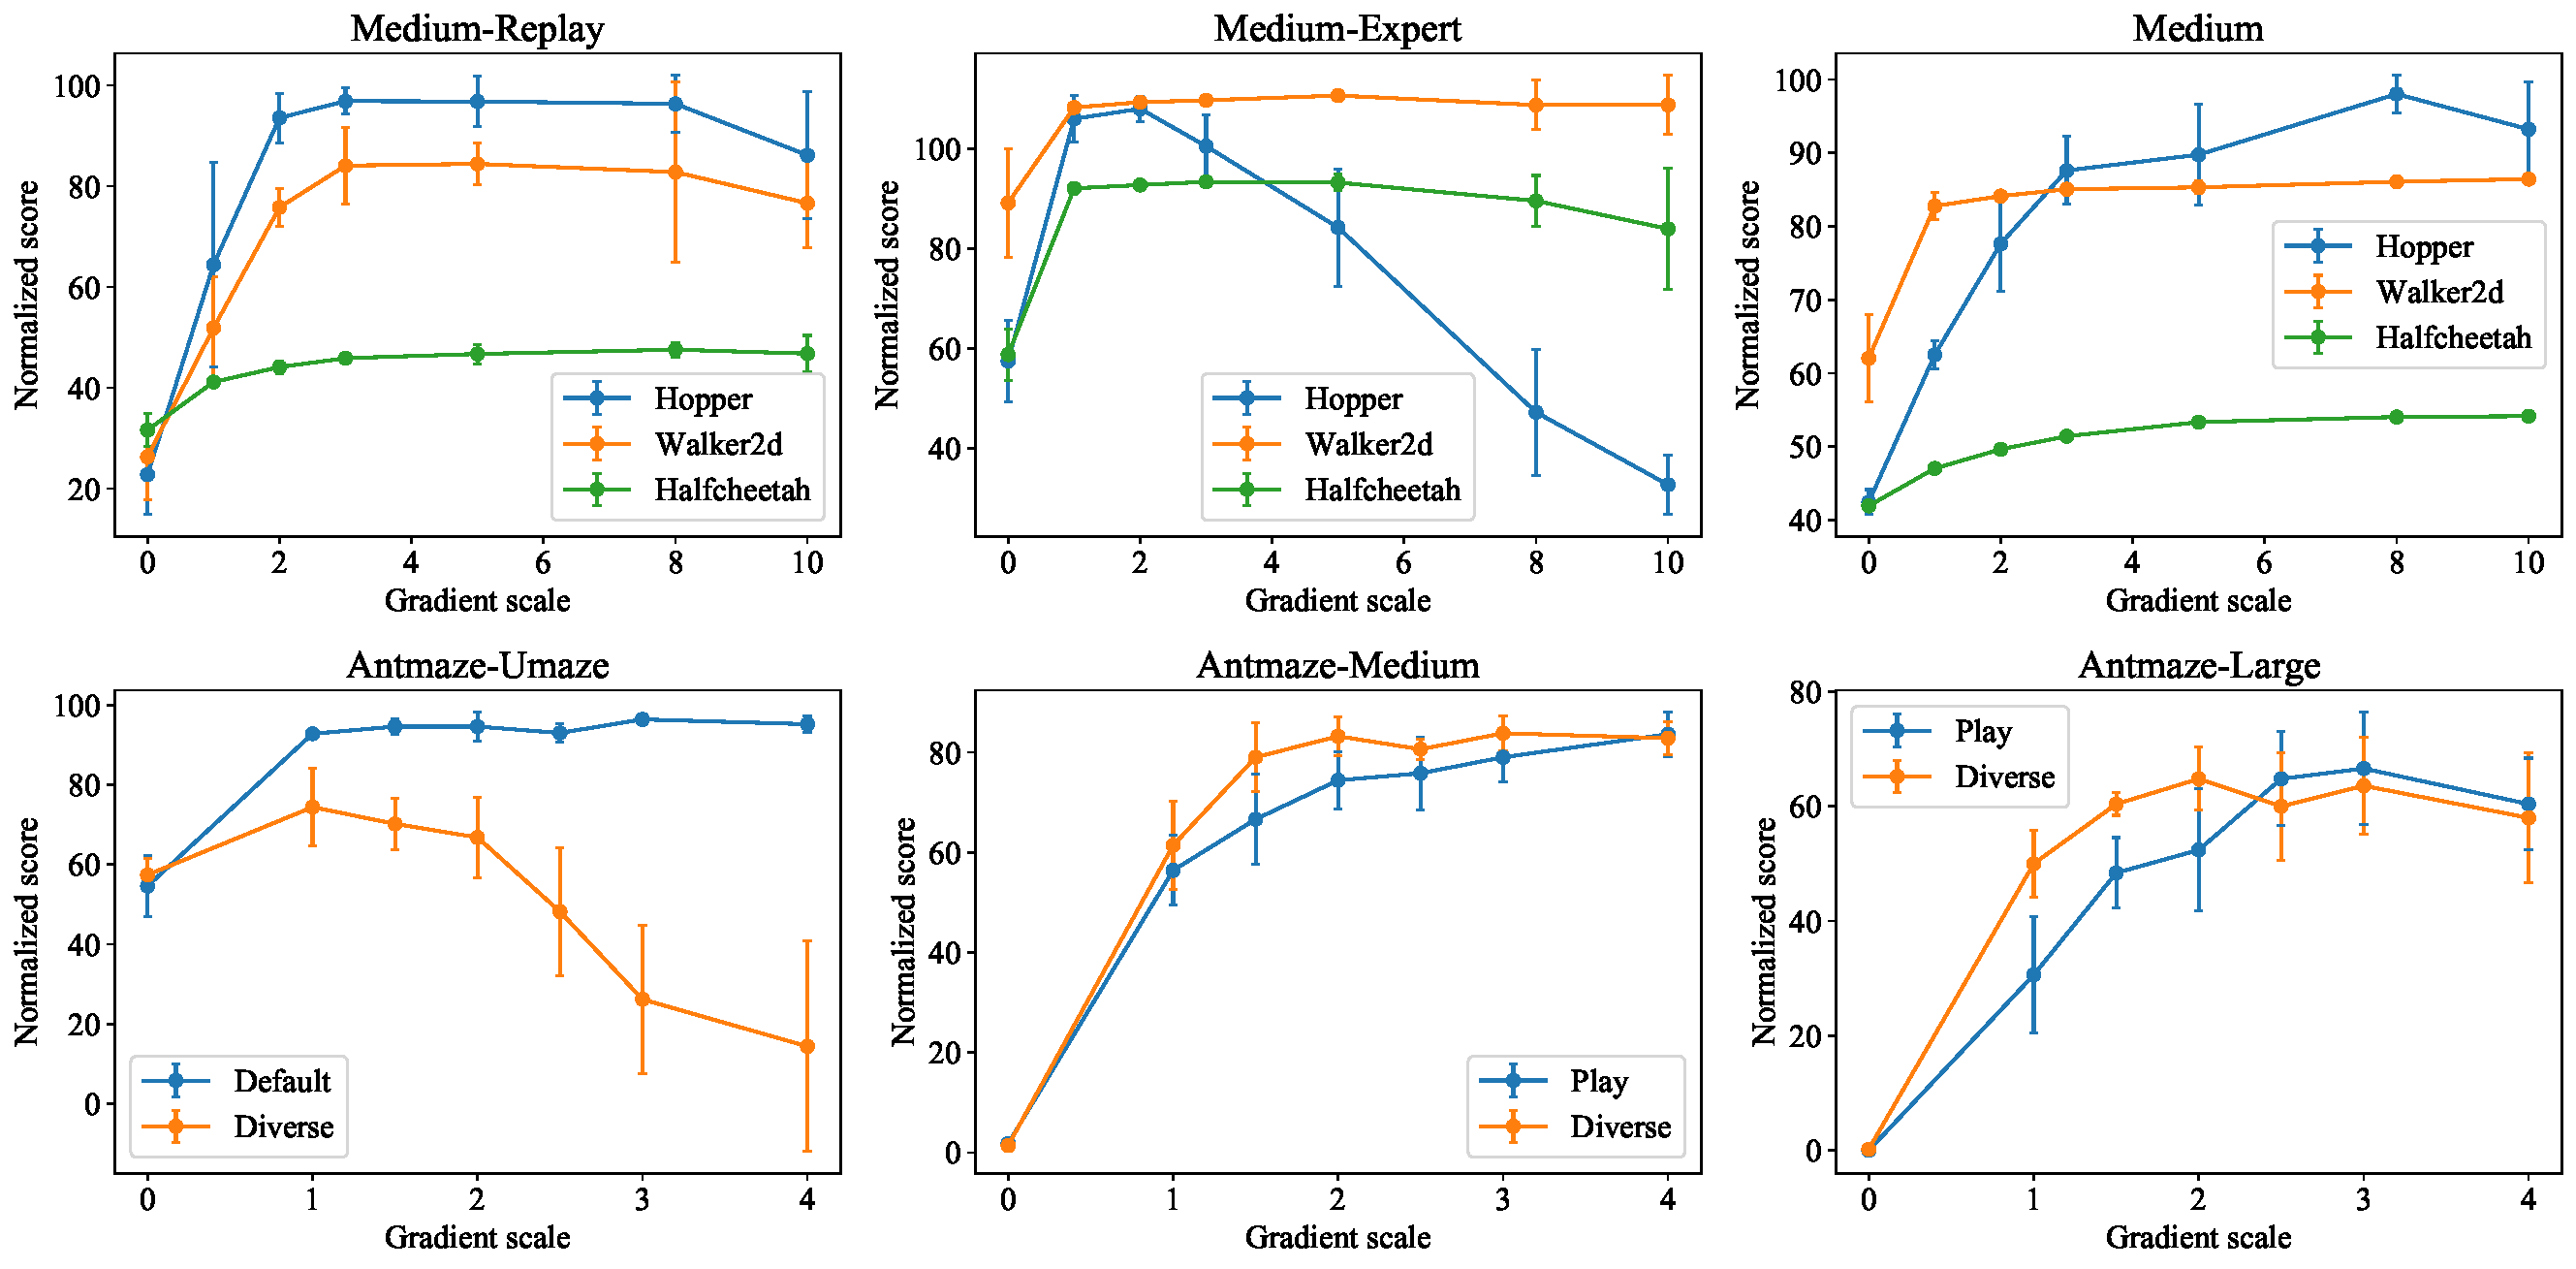
\includegraphics[width=\linewidth]{pics/gradient_scale_all.pdf}
\caption{
Ablation of gradient scales in D4RL benchmark.
}
\label{fig:ablation_gradient_scale}
\end{figure}

\begin{figure}[h]
\centering
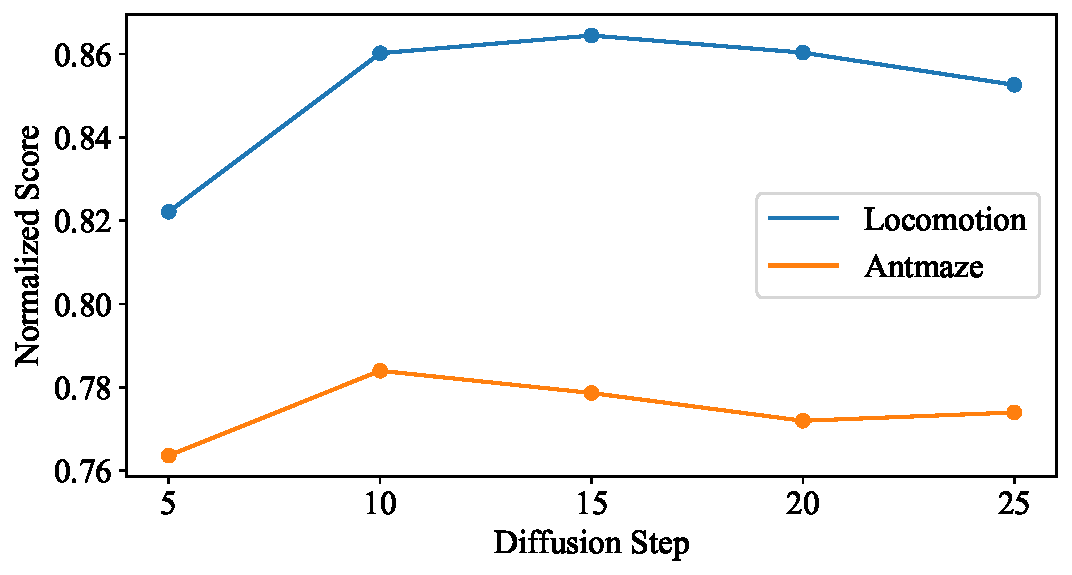
\includegraphics[width=0.5\linewidth]{pics/ablate_ds.pdf}

\caption{
Ablation of diffusion steps in evaluation.
}
\label{fig:ablation_diffusion_steps}
\end{figure}

\begin{table}[h]
\centering
\begin{tabular}{c|c|c|c}
\hline
\multirow{2}*{Locomotion-Medium-Expert} & Walker2d & Halfcheetah & Hopper\\
~ & 5.0 & 3.0 & 2.0\\
\hline
\multirow{2}*{Locomotion-Medium} & Walker2d & Halfcheetah & Hopper\\
~ & 10.0 & 10.0 & 8.0\\
\hline
\multirow{2}*{Locomotion-Medium-Replay} & Walker2d & Halfcheetah & Hopper\\
~ & 5.0 & 8.0 & 3.0\\
\hline    
\multirow{2}*{AntMaze-Fixed} & Umaze & Medium & Large\\
~ & 3.0 & 4.0 & 3.0\\
\hline
\multirow{2}*{AntMaze-Diverse} & Umaze & Medium & Large\\
~ & 1.0 & 3.0 & 2.0\\
\hline
\end{tabular}
\caption{Guidance scale $s$ used across different tasks}
\label{tbl:gradient_scales_rl}
\end{table}



\subsection{Experiment Details for Other Baselines}
\label{appendix:RL_baselines}
\paragraph{Diffusion-QL.}
We use the official implementation of Diffusion-QL ( \url{https://github.com/Zhendong-Wang/Diffusion-Policies-for-Offline-RL}) and default hyperparameter settings to rerun all experiments for Diffusion-QL to ensure a consistent evaluation metric. We follow \citet{d4rl} and report averaged scores across 5 independent trails at the end of training for each task, instead of the max performance scores during training as in \citet{dql}. In addition, we notice that Diffusion-QL adopts a resampling technique for evaluation. Specifically, during evaluation, the learned policy first generates 50 different action candidates and then selects one action with the highest Q-value for execution. We empirically found that such a technique is important for good performance in MuJoCo Locomotion tasks. However, this technique makes it hard to reflect the true quality of sampled actions before resampling and is computationally expensive, we thus additionally conduct an ablation study in which we remove the resampling procedure in evaluation, and use a single action candidate (Diffusion-QL@1 in \cref{tbl:rl_results} and \cref{sec:training_curves}). 

\paragraph{Ablations of CEP guidance.}
We study three variations of our proposed guidance method. Specifically, an MSE-based guidance method as described in \eqref{Eq:MSE_qt_objective} (similarly used in \citet{diffuser}), an E-MSE guidance method as described in \eqref{Eq:emse}, and a resampling-based method following \citet{sfbc}. For MSE and E-MSE guidance, we only change the training objective of the energy guidance model while leaving other hyperparameters untouched. For the resampling-based method, the energy guidance model is not required. During evaluation, at every decision step we first sample 50 random action candidates from the behavior policy model $\mu_\theta(\va|\vs)$ and then select one action with the highest predicted Q-value via $Q_\psi$ for execution.

\begin{table}[]
    \centering
    \begin{tabular}{lcccc}
        \toprule
        \textbf{Environment} & \textbf{MSE}& \textbf{E-MSE} & \textbf{RS} & \textbf{CEP} \\
        \midrule
        \textbf{Locomotion} & $68.0$  & $58.1$ & $76.9$  & $86.6$\\ 
        \textbf{AntMaze} & $46.4$ & $24.5$ & $63.0$ & $78.3$ \\ 
        \bottomrule
    \end{tabular}
    \caption{Ablation studies of different energy guidance methods and the resampling technique.}
    \label{tab:Ablation_RL}
\end{table}











\section{Experiment Details for 2-D experiments}
To perform unconditional energy-guided sampling in low-dimensional data space. Our method requires training two neural networks independently, specifically, one generative diffusion model and one energy guidance model. In contrast with offline RL, the energy function at $t=0$ data space is pre-defined (as illustrated in \cref{fig:toy_appendix}) and does not require training. A total of 1M datapoints is generated and used as the training set. Each datapoint contains a two-dimensional data sample $\x$ and a float number $e$ representing its energy.

\paragraph{Training diffusion generative models.}
The generative diffusion model is a 5-layer MLP with hidden sizes of $[512, 512, 512, 512, 256]$ and SiLU activations. The network is trained for 750 epochs, using the Adam optimizer with a learning rate of 1e-4. The batchsize is 1 with $K=4096$. As for the data perturbation method, we adopt the default VPSDE setting in \citep{song2020score} with a linear schedule. The $\alpha_t$ and $\sigma_t$ in \eqref{Eq:forward_p} are:
\begin{equation}
    \alpha_t = -\frac{\beta_1 - \beta_0}{4}t^2 - \frac{\beta_0}{2}t, \quad \sigma_t = \sqrt{1 - \alpha_t^2}, \quad \beta_0=0.1,\ \beta_1=20.
\end{equation}


\paragraph{Training energy guidance models.}
The energy guidance model is a 4-layer MLP with 512 hidden units and SiLU activations. We train it for 750 epochs, using the Adam optimizer with a learning rate of 3e-4. The batchsize is also 4096.

\paragraph{Guided sampling.}
 In order to perform guided sampling, we adopt a recent advance in diffusion sampling, namely DPM-Solver \citep{lu2022dpm}. We use the second-order sampler and a diffusion step of 25. We fix the guidance scale $s$ to 1 in all experiments.

\section{Experiment Details for Image Synthesis}
We completely follow \citet{diffusion_beat_gan} to train and evaluate our energy-guided diffusion models for image synthesis, without any kind of hyperparameter tuning or network architecture changes. For the generative diffusion prior, we use the pretrained ImageNet models released at \url{https://github.com/openai/guided-diffusion}. For the energy guidance model, we adopt the same U-Net architecture as \citet{diffusion_beat_gan} but rewrite the training objective to \eqref{Eq:contarstive_condition_loss} for conditional image synthesis, and to \eqref{Eq:infoNCE_energy_normalized} for energy guided image synthesis. Our ImageNet 128 energy guidance model is trained for 300k gradient steps with a batch size of 256 (distributed on 8 GPUs). The ImageNet 256 energy guidance model is trained for 500k steps. During sampling, we use 250 diffusion steps by default except when we use a DDIM \citep{song2020denoising} sampler with 25 steps. 

For energy-guided image synthesis tasks, we set $\beta=50$. A penalty is added to the energy function at defined $t=0$ data space in \eqref{Eq:color_q0} when the image's average saturation is lower than $0.1$. This penalization mainly intends to avoid generating images with low saturation (overly bright), such that image samples guided by different color models are more distinguishable. We respectively let $h_\text{tar}$ be $0$ (red), $2\pi/3$ (green) and $4\pi/3$ (blue) for the three guidance models.

\newpage
\section{More 2-D Results}
\label{appendix:toy_more}

\begin{figure}[!hbt]
\centering
\begin{minipage}{0.03\linewidth}
\rotatebox{90}{\scriptsize{Groundtruth}}
\end{minipage}
\begin{minipage}{0.46\linewidth}
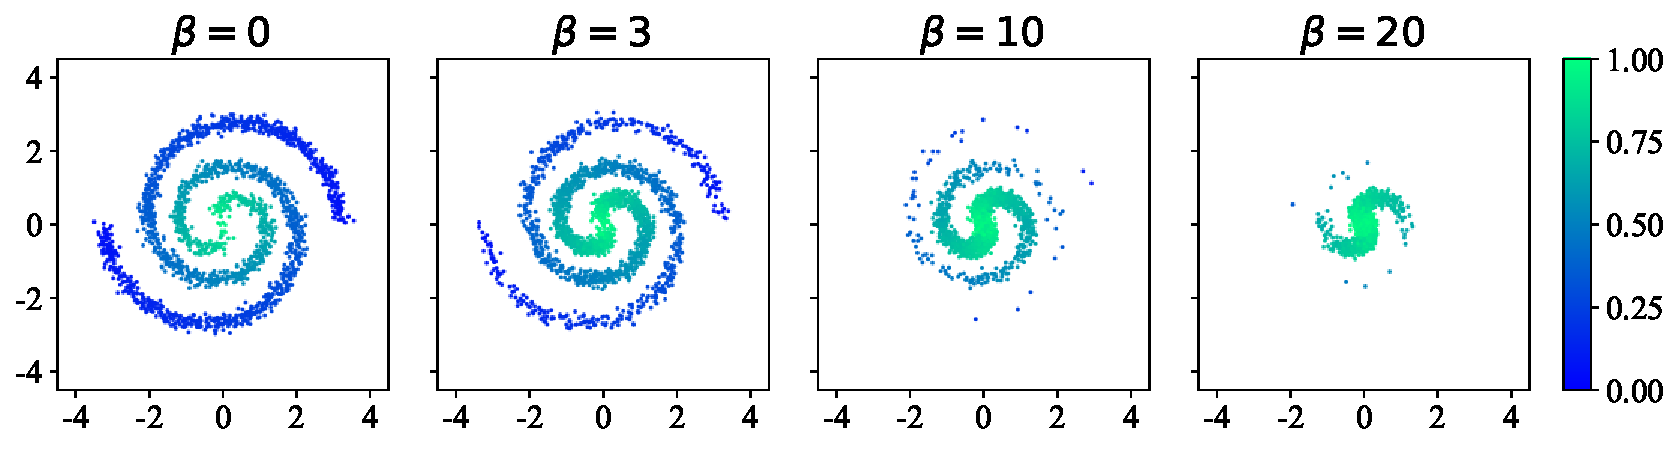
\includegraphics[width=\columnwidth]{pics/toy_scatter/2spirals_groudtruth.pdf}
\end{minipage}
\begin{minipage}{0.46\linewidth}
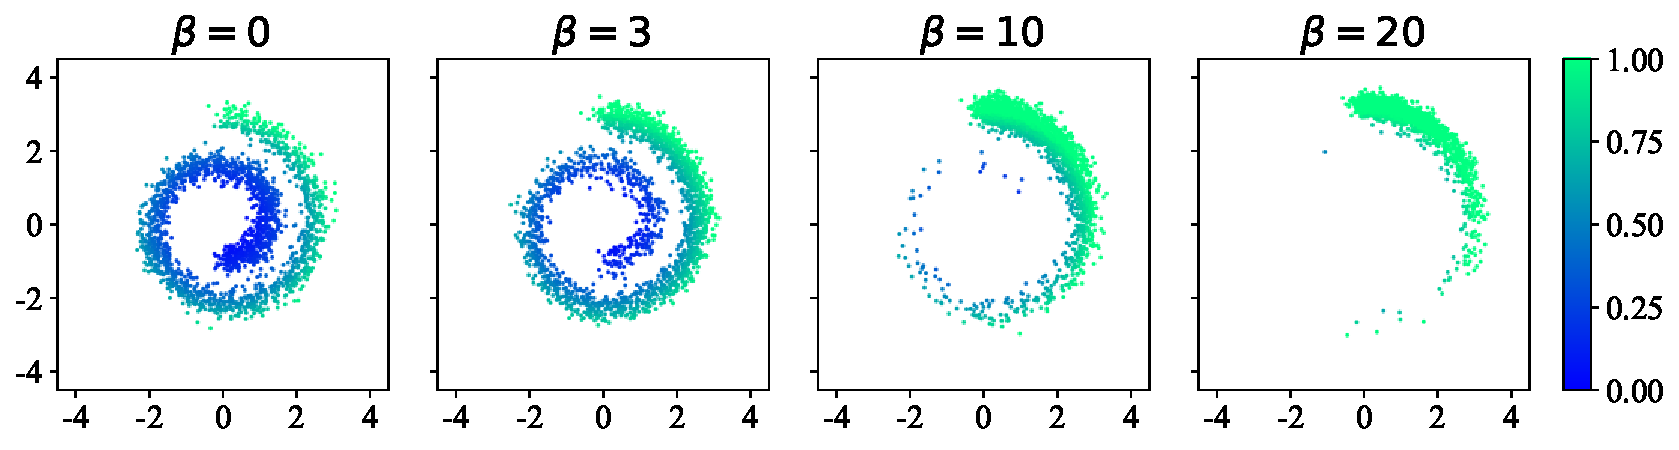
\includegraphics[width=\columnwidth]{pics/toy_scatter/swissroll_groudtruth.pdf}
\end{minipage}\\
\begin{minipage}{0.015\linewidth}
\rotatebox{90}{\scriptsize{DPS}}
\end{minipage}
\begin{minipage}{0.015\linewidth}
\rotatebox{90}{\scriptsize{(\citeauthor{chung2022diffusion}, etc.)}}
\end{minipage}
\begin{minipage}{0.46\linewidth}
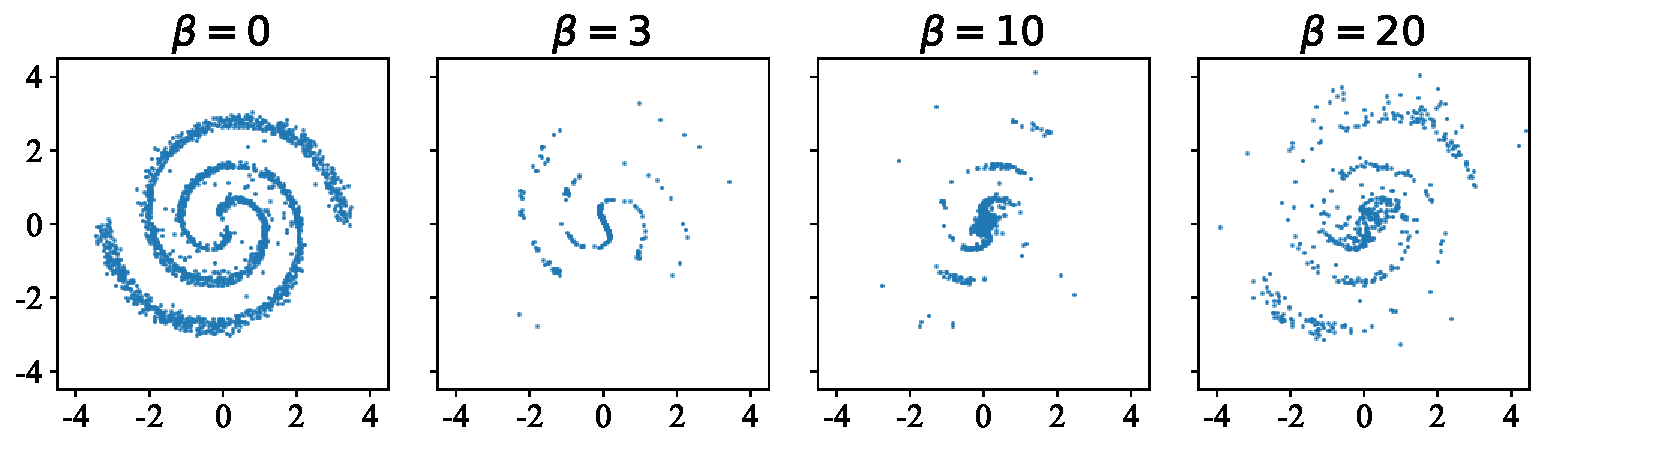
\includegraphics[width=\columnwidth]{pics/toy_scatter/2spirals_DPS.pdf}
\end{minipage}
\begin{minipage}{0.46\linewidth}
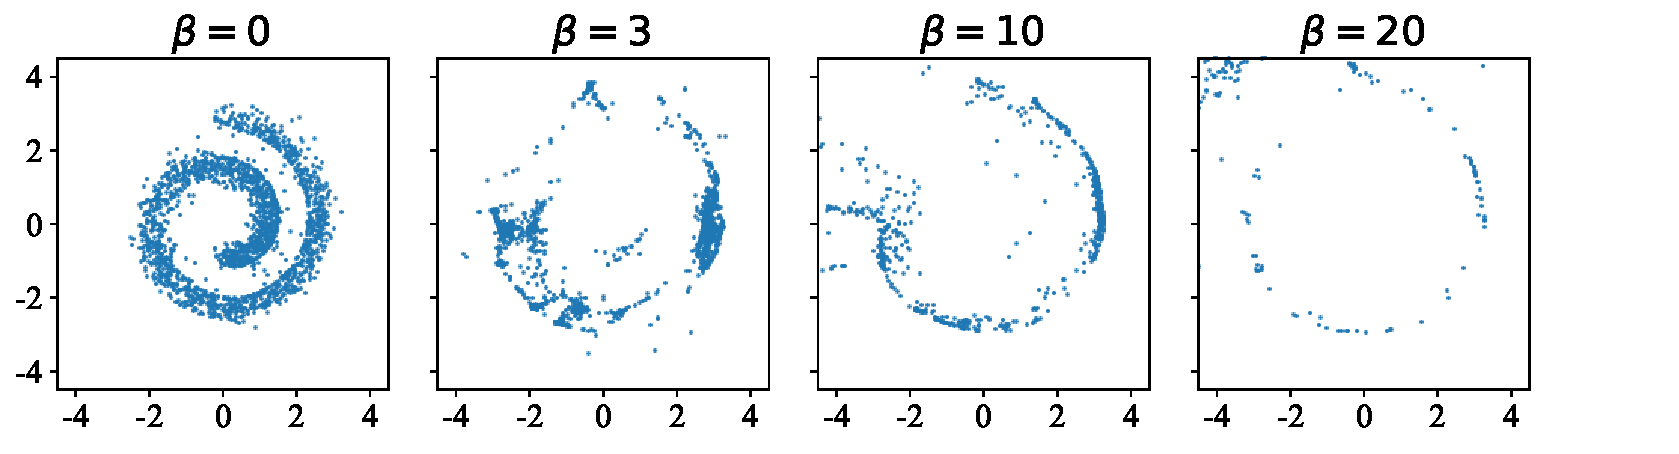
\includegraphics[width=\columnwidth]{pics/toy_scatter/swissroll_DPS.pdf}
\end{minipage}\\
\begin{minipage}{0.015\linewidth}
\rotatebox{90}{\scriptsize{MSE}}
\end{minipage}
\begin{minipage}{0.015\linewidth}
\rotatebox{90}{\scriptsize{(\citeauthor{diffuser}, etc.)}}
\end{minipage}
\begin{minipage}{0.46\linewidth}
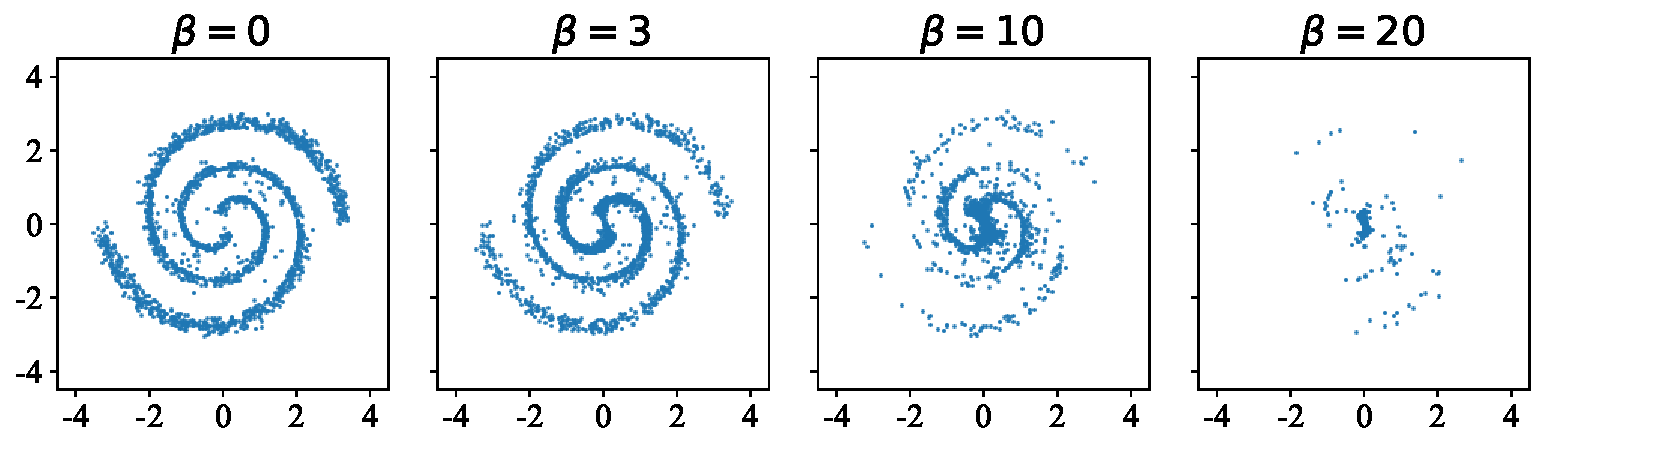
\includegraphics[width=\columnwidth]{pics/toy_scatter/2spirals_mse.pdf}
\end{minipage}
\begin{minipage}{0.46\linewidth}
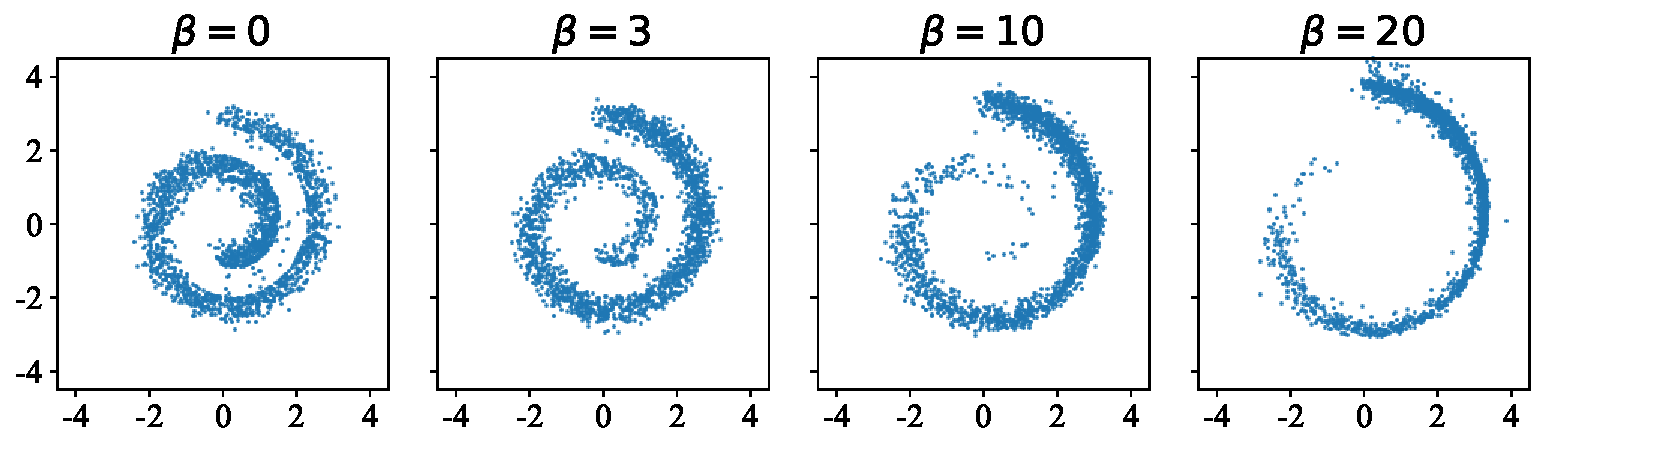
\includegraphics[width=\columnwidth]{pics/toy_scatter/swissroll_mse.pdf}
\end{minipage}\\
\begin{minipage}{0.015\linewidth}
\rotatebox{90}{\scriptsize{E-MSE}}
\end{minipage}
\begin{minipage}{0.015\linewidth}
\rotatebox{90}{\scriptsize{(\textbf{ours})}}
\end{minipage}
\begin{minipage}{0.46\linewidth}
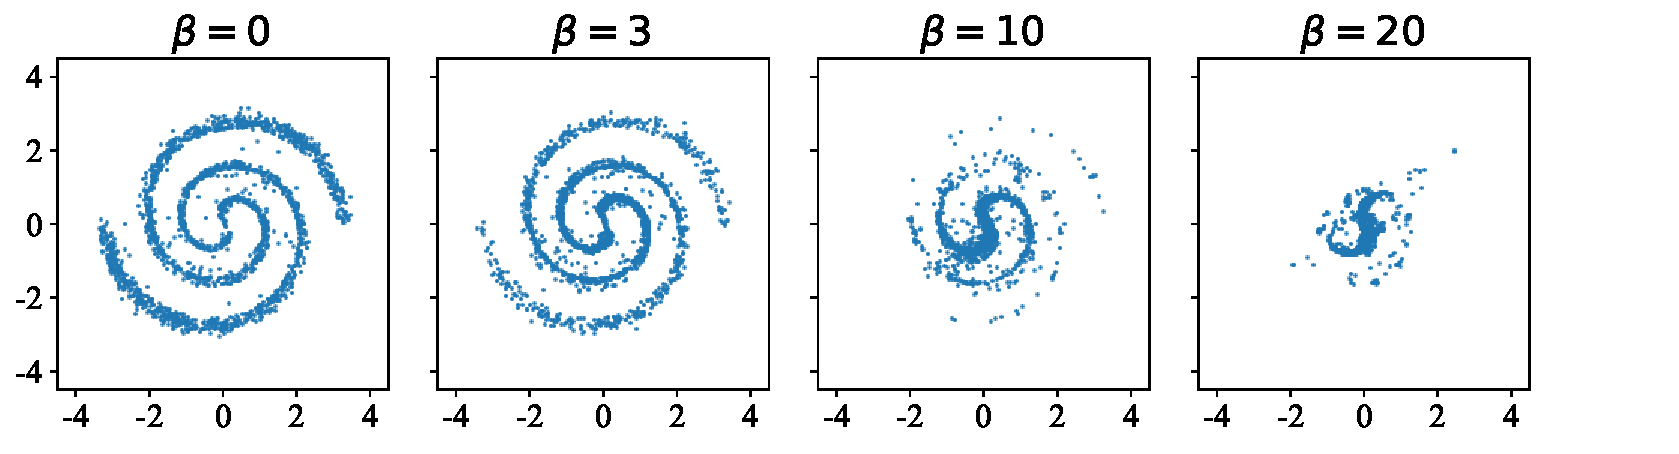
\includegraphics[width=\columnwidth]{pics/toy_scatter/2spirals_emse.pdf}
\end{minipage}
\begin{minipage}{0.46\linewidth}
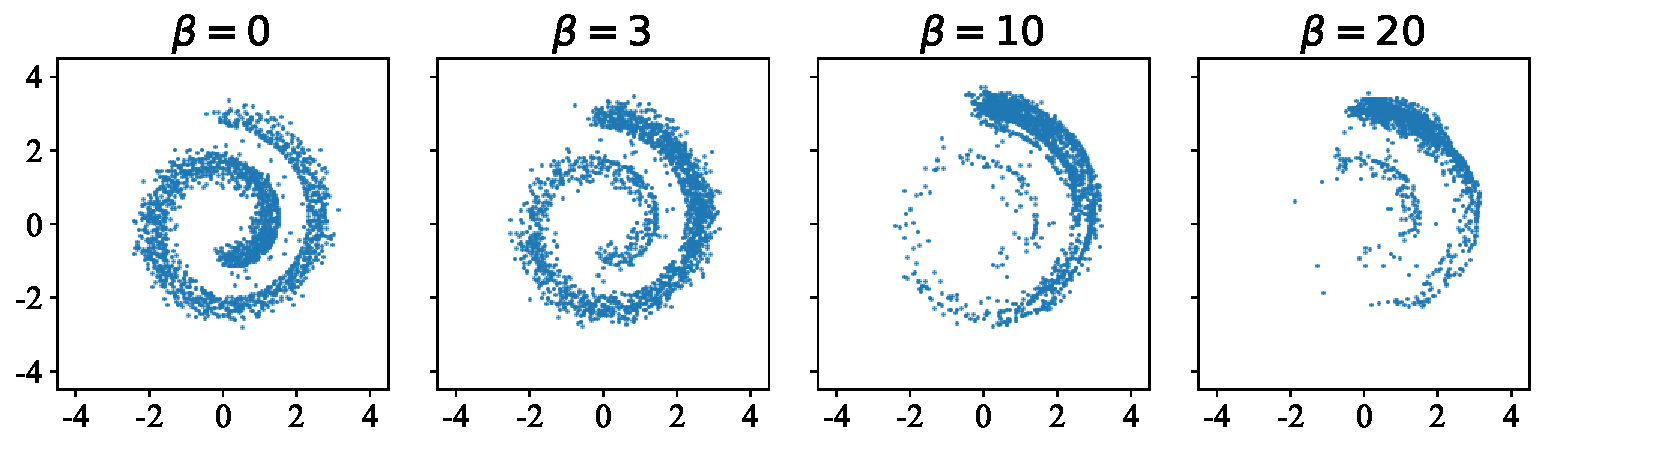
\includegraphics[width=\columnwidth]{pics/toy_scatter/swissroll_emse.pdf}
\end{minipage}\\
\begin{minipage}{0.015\linewidth}
\rotatebox{90}{\scriptsize{CEP}}
\end{minipage}
\begin{minipage}{0.015\linewidth}
\rotatebox{90}{\scriptsize{(\textbf{ours})}}
\end{minipage}
\begin{minipage}{0.46\linewidth}
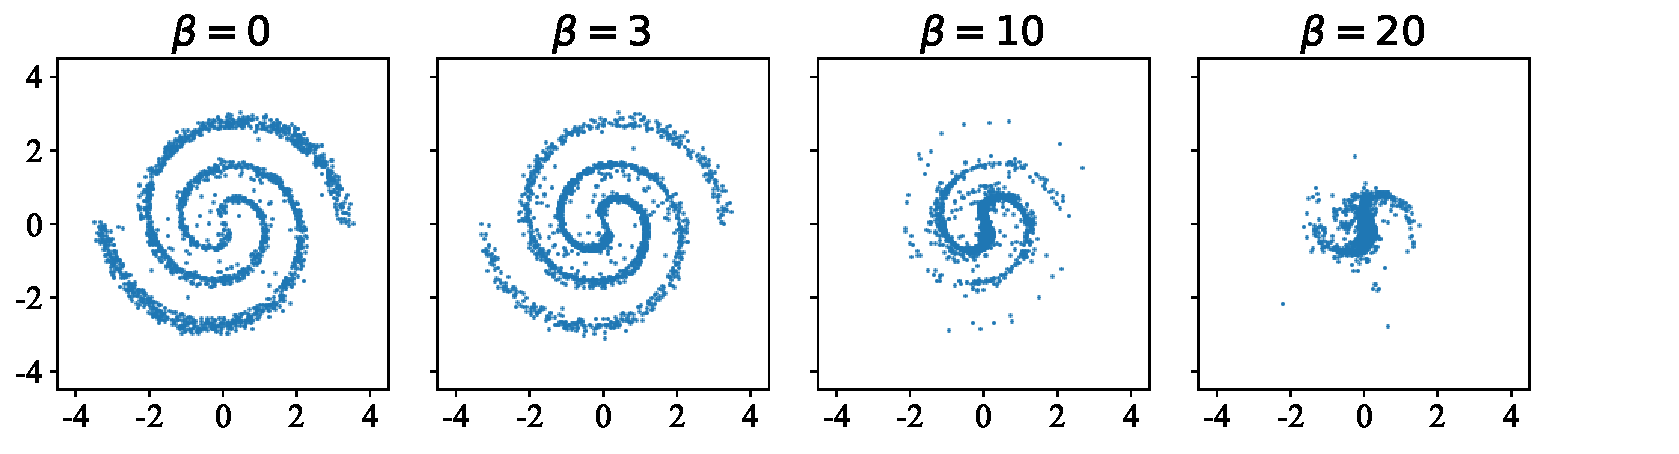
\includegraphics[width=\columnwidth]{pics/toy_scatter/2spirals_cross_entrophy.pdf}
\end{minipage}
\begin{minipage}{0.46\linewidth}
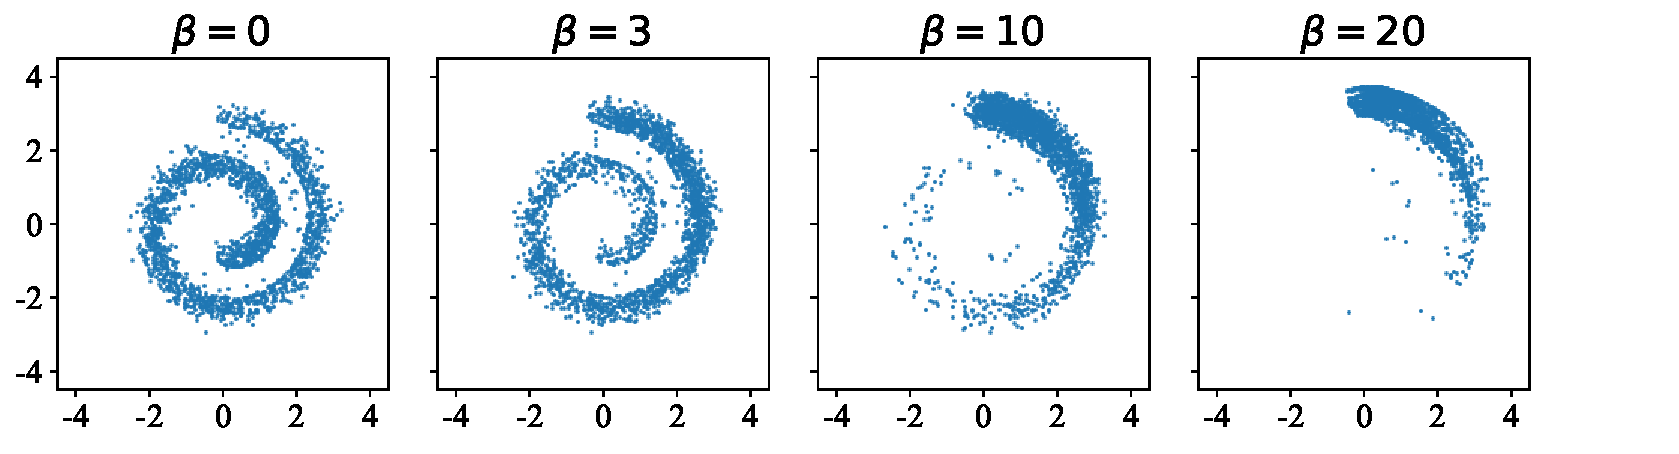
\includegraphics[width=\columnwidth]{pics/toy_scatter/swissroll_cross_entrophy.pdf}
\end{minipage}\\
\begin{minipage}{0.03\linewidth}
\rotatebox{90}{\scriptsize{Groundtruth}}
\end{minipage}
\begin{minipage}{0.46\linewidth}
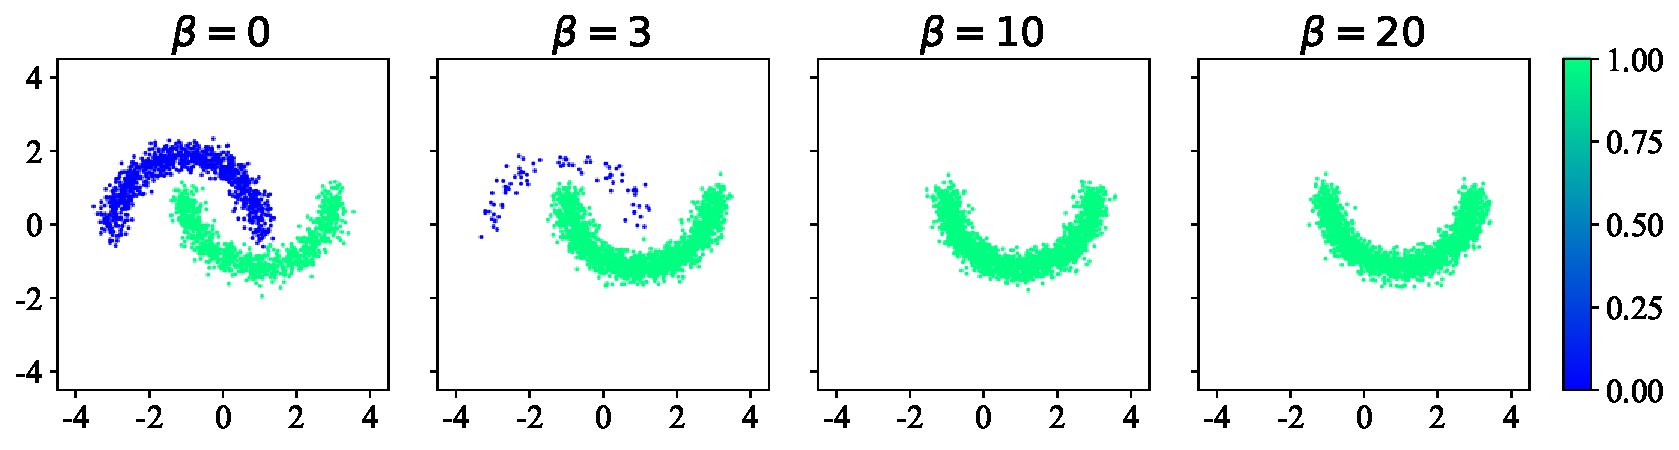
\includegraphics[width=\columnwidth]{pics/toy_scatter/moons_groudtruth.pdf}
\end{minipage}
\begin{minipage}{0.46\linewidth}
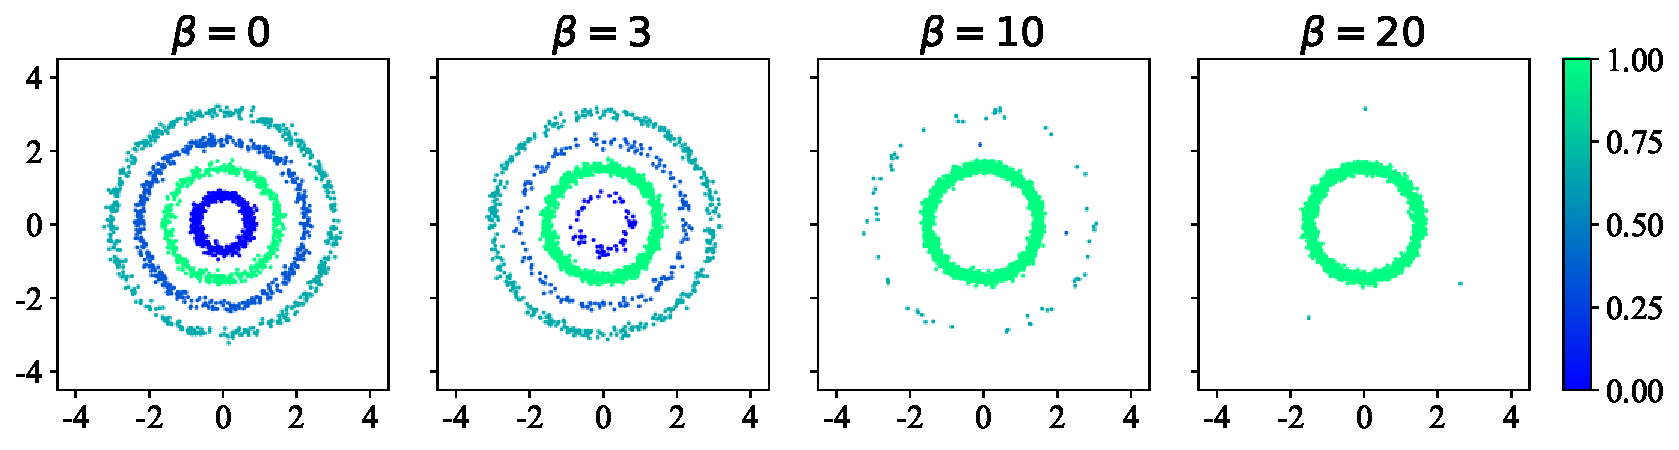
\includegraphics[width=\columnwidth]{pics/toy_scatter/rings_groudtruth.pdf}
\end{minipage}\\
\begin{minipage}{0.015\linewidth}
\rotatebox{90}{\scriptsize{DPS}}
\end{minipage}
\begin{minipage}{0.015\linewidth}
\rotatebox{90}{\scriptsize{(\citeauthor{chung2022diffusion}, etc.)}}
\end{minipage}
\begin{minipage}{0.46\linewidth}
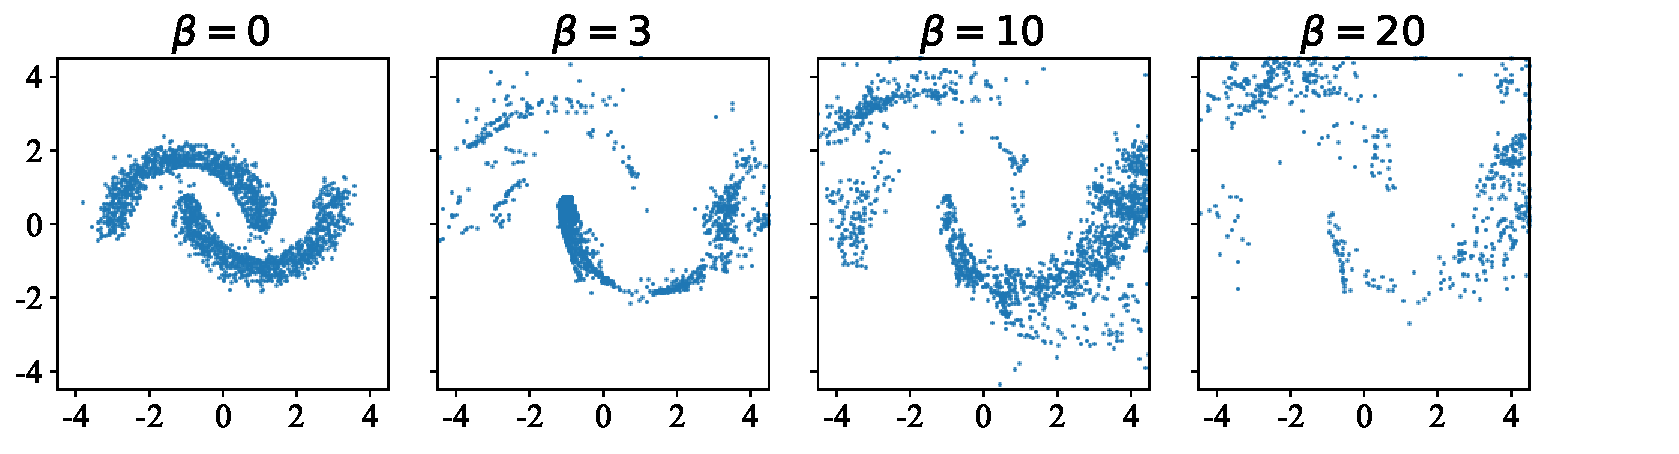
\includegraphics[width=\columnwidth]{pics/toy_scatter/moons_DPS.pdf}
\end{minipage}
\begin{minipage}{0.46\linewidth}
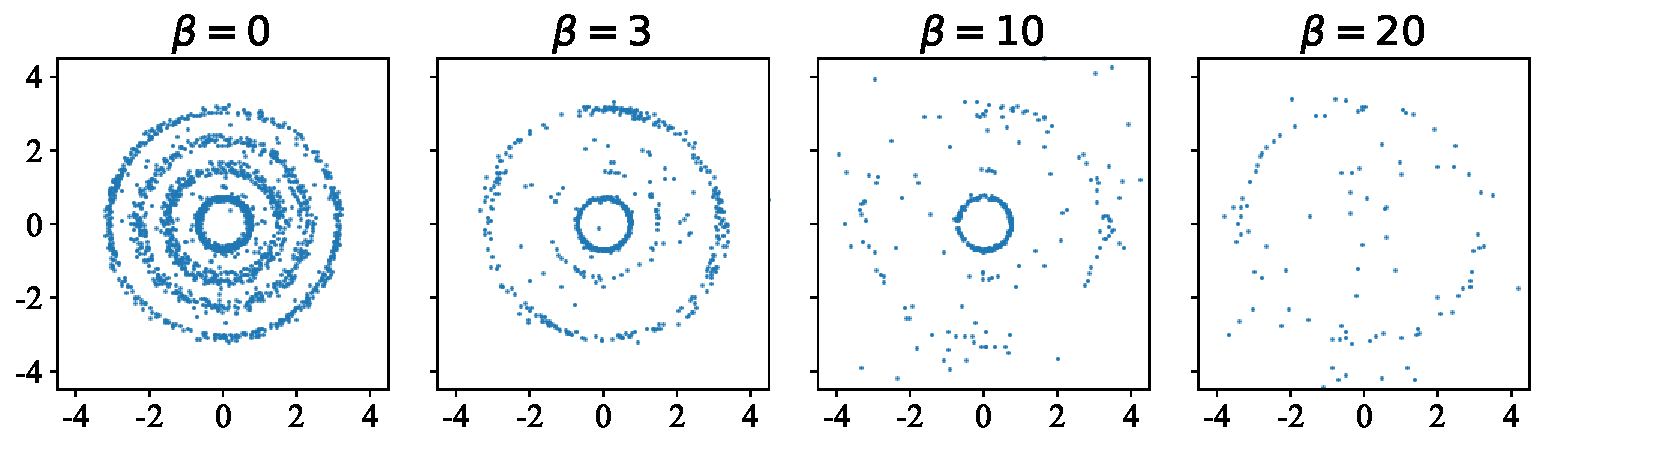
\includegraphics[width=\columnwidth]{pics/toy_scatter/rings_DPS.pdf}
\end{minipage}\\
\begin{minipage}{0.015\linewidth}
\rotatebox{90}{\scriptsize{MSE}}
\end{minipage}
\begin{minipage}{0.015\linewidth}
\rotatebox{90}{\scriptsize{(\citeauthor{diffuser}, etc.)}}
\end{minipage}
\begin{minipage}{0.46\linewidth}
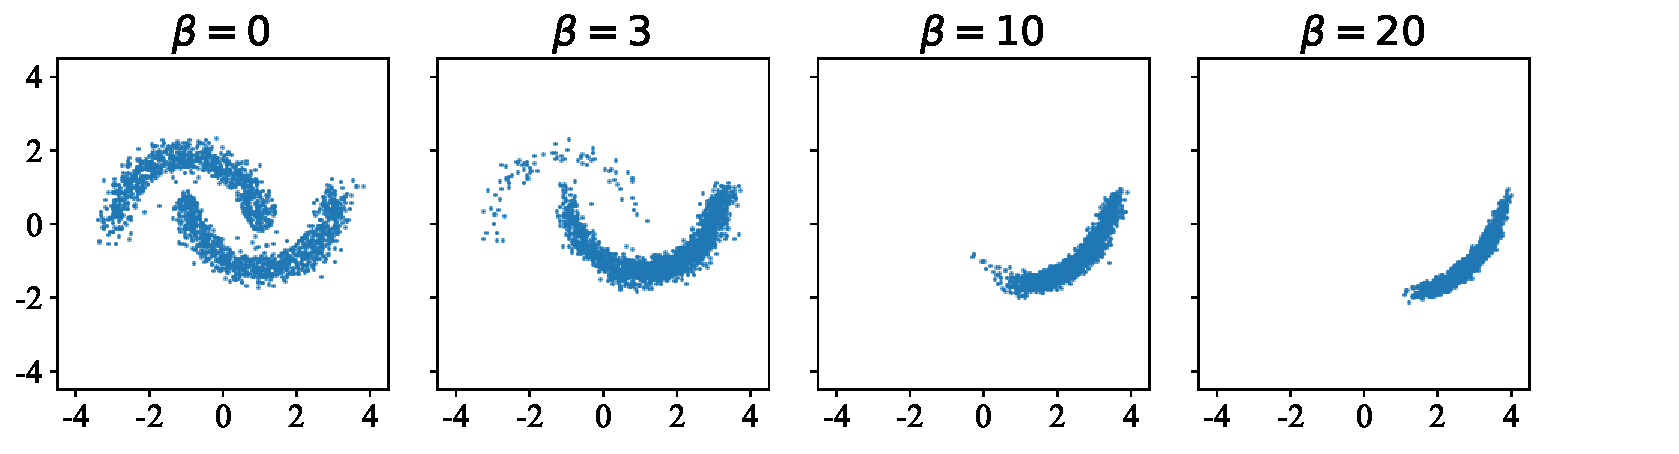
\includegraphics[width=\columnwidth]{pics/toy_scatter/moons_mse.pdf}
\end{minipage}
\begin{minipage}{0.46\linewidth}
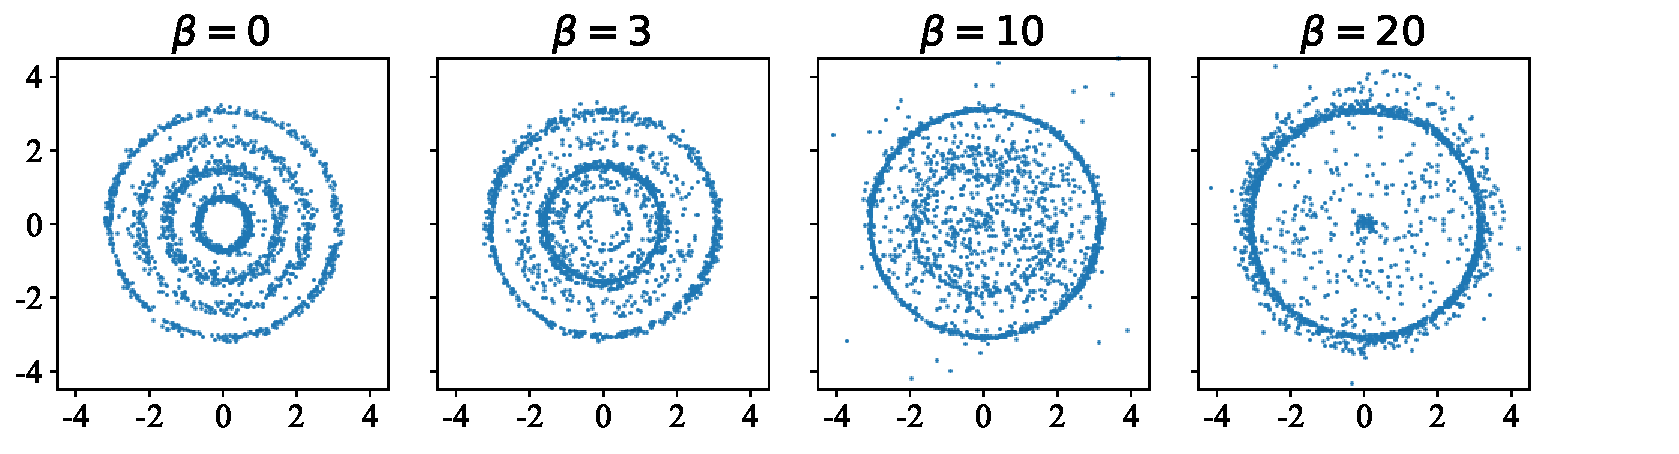
\includegraphics[width=\columnwidth]{pics/toy_scatter/rings_mse.pdf}
\end{minipage}\\
\begin{minipage}{0.015\linewidth}
\rotatebox{90}{\scriptsize{E-MSE}}
\end{minipage}
\begin{minipage}{0.015\linewidth}
\rotatebox{90}{\scriptsize{(\textbf{ours})}}
\end{minipage}
\begin{minipage}{0.46\linewidth}
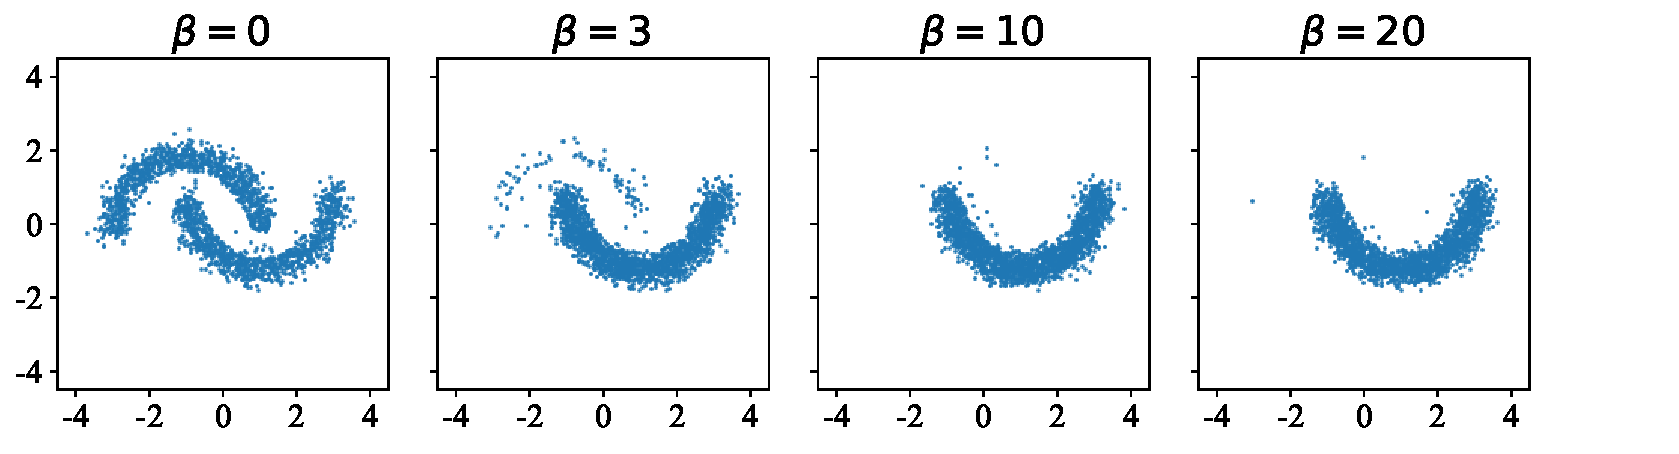
\includegraphics[width=\columnwidth]{pics/toy_scatter/moons_emse.pdf}
\end{minipage}
\begin{minipage}{0.46\linewidth}
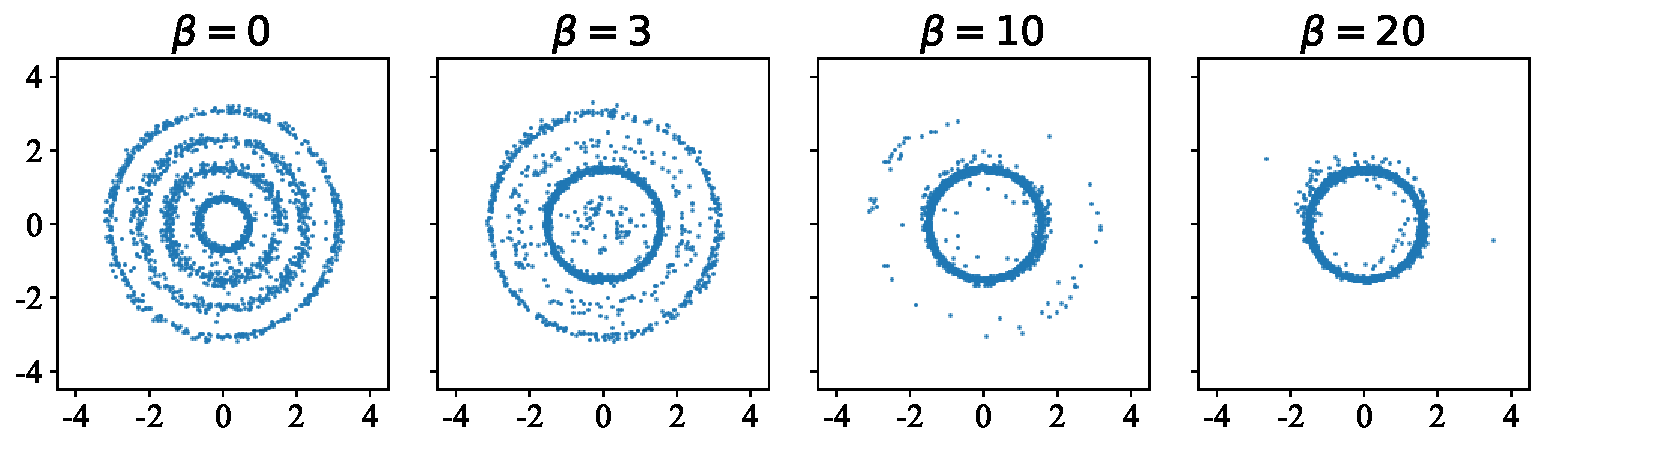
\includegraphics[width=\columnwidth]{pics/toy_scatter/rings_emse.pdf}
\end{minipage}\\
\begin{minipage}{0.015\linewidth}
\rotatebox{90}{\scriptsize{CEP}}
\end{minipage}
\begin{minipage}{0.015\linewidth}
\rotatebox{90}{\scriptsize{(\textbf{ours})}}
\end{minipage}
\begin{minipage}{0.46\linewidth}
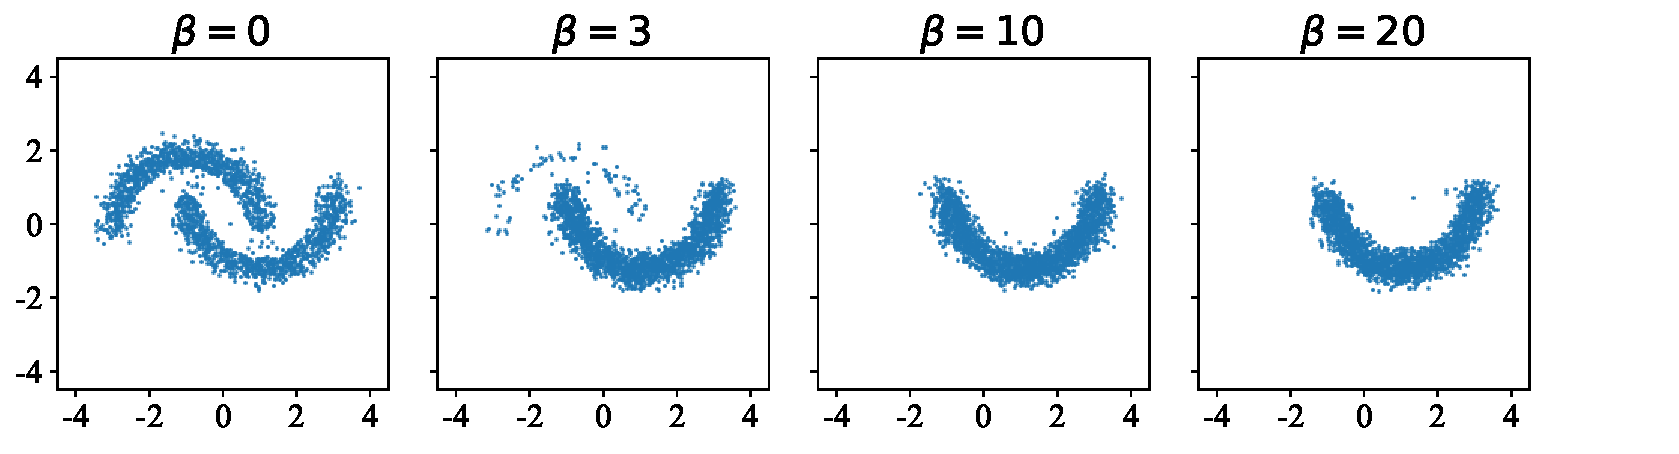
\includegraphics[width=\columnwidth]{pics/toy_scatter/moons_cross_entrophy.pdf}
\end{minipage}
\begin{minipage}{0.46\linewidth}
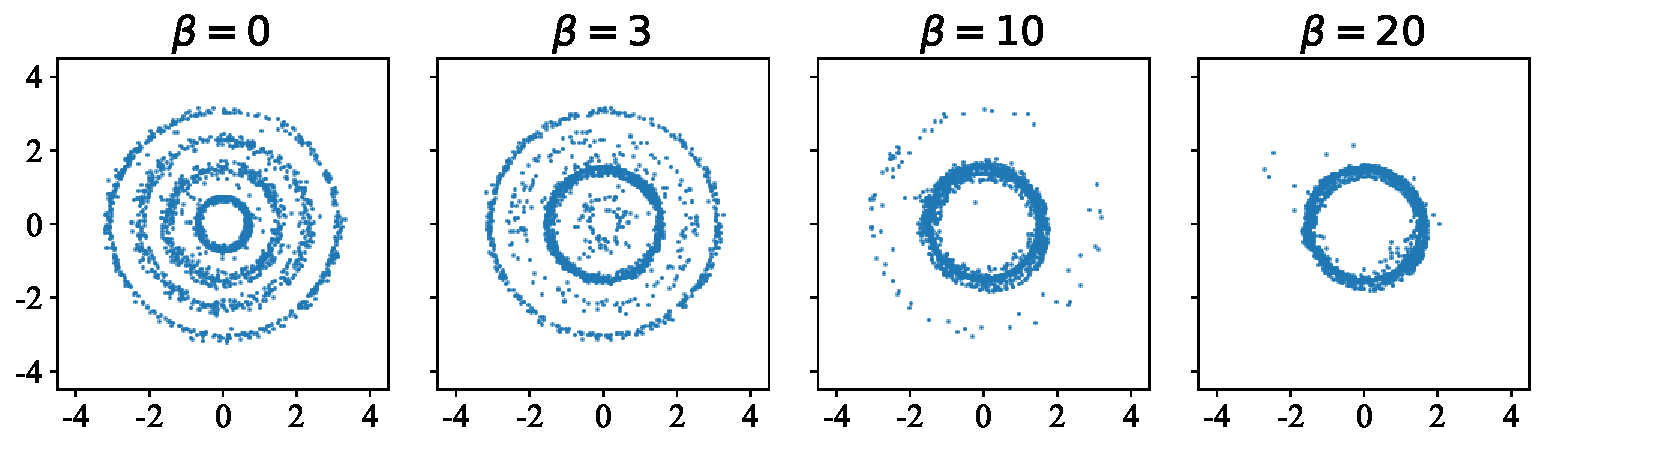
\includegraphics[width=\columnwidth]{pics/toy_scatter/rings_cross_entrophy.pdf}
\end{minipage}\\
\caption{
Scatter plots of different energy guidance methods in 2-D experiments. E-MSE is another method we propose as a variant of MSE guidance (\cref{sec:emse}).
}
\vspace{-8mm}
\label{fig:toy_appendix}
\end{figure}

\newpage
\begin{figure}[!hbt]
\centering
\begin{minipage}{0.02\linewidth}
\rotatebox{90}{\scriptsize{8gaussians}}
\end{minipage}
\begin{minipage}{0.97\linewidth}
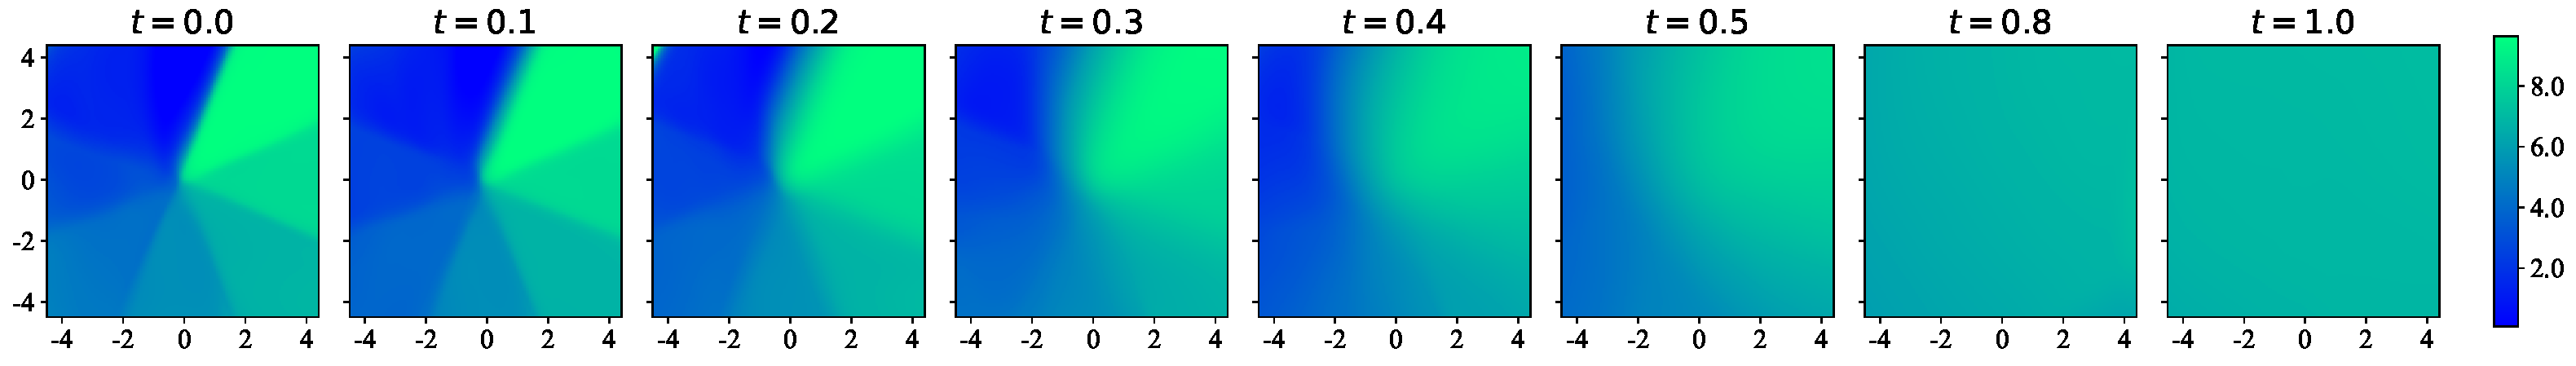
\includegraphics[width=\columnwidth]{pics/toy_scatter/8gaussians_qt.pdf}
\end{minipage}\\
\begin{minipage}{0.02\linewidth}
\rotatebox{90}{\scriptsize{swissroll}}
\end{minipage}
\begin{minipage}{0.97\linewidth}
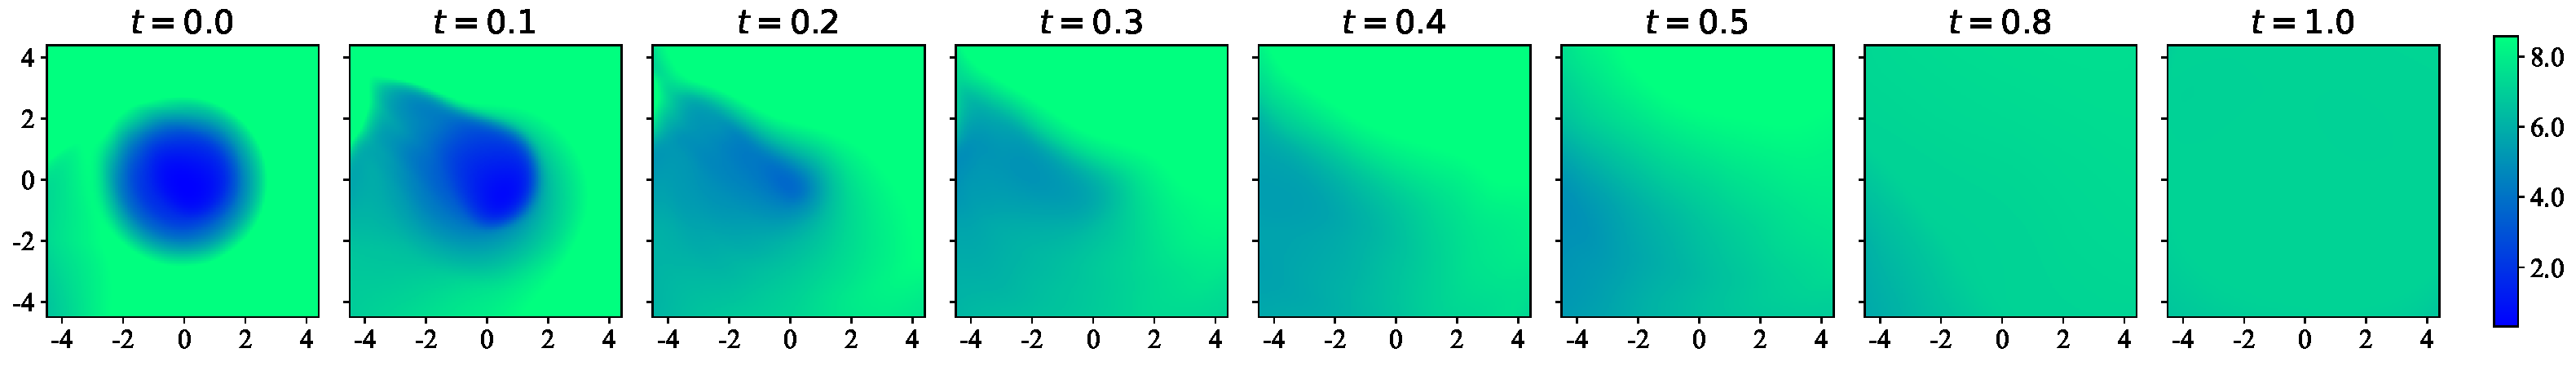
\includegraphics[width=\columnwidth]{pics/toy_scatter/swissroll_qt.pdf}
\end{minipage}\\
\begin{minipage}{0.02\linewidth}
\rotatebox{90}{\scriptsize{2spirals}}
\end{minipage}
\begin{minipage}{0.97\linewidth}
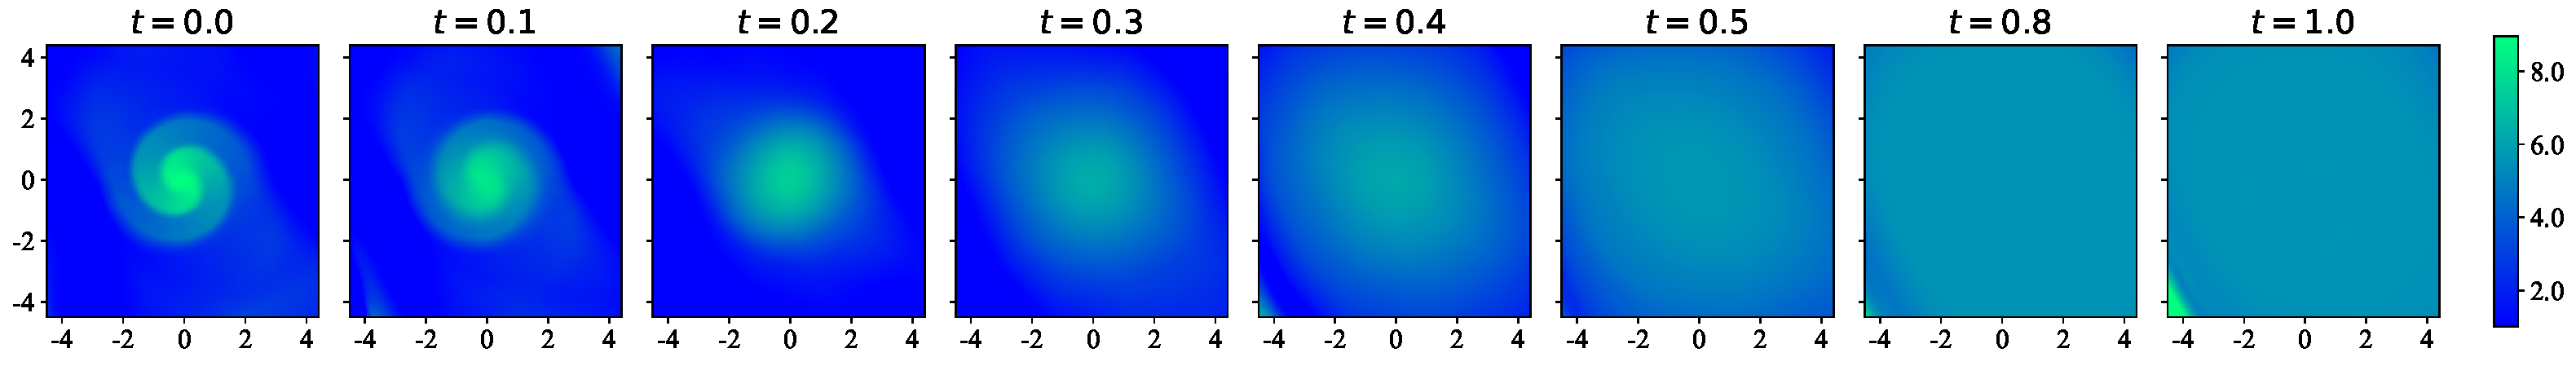
\includegraphics[width=\columnwidth]{pics/toy_scatter/2spirals_qt.pdf}
\end{minipage}\\
\begin{minipage}{0.02\linewidth}
\rotatebox{90}{\scriptsize{moons}}
\end{minipage}
\begin{minipage}{0.97\linewidth}
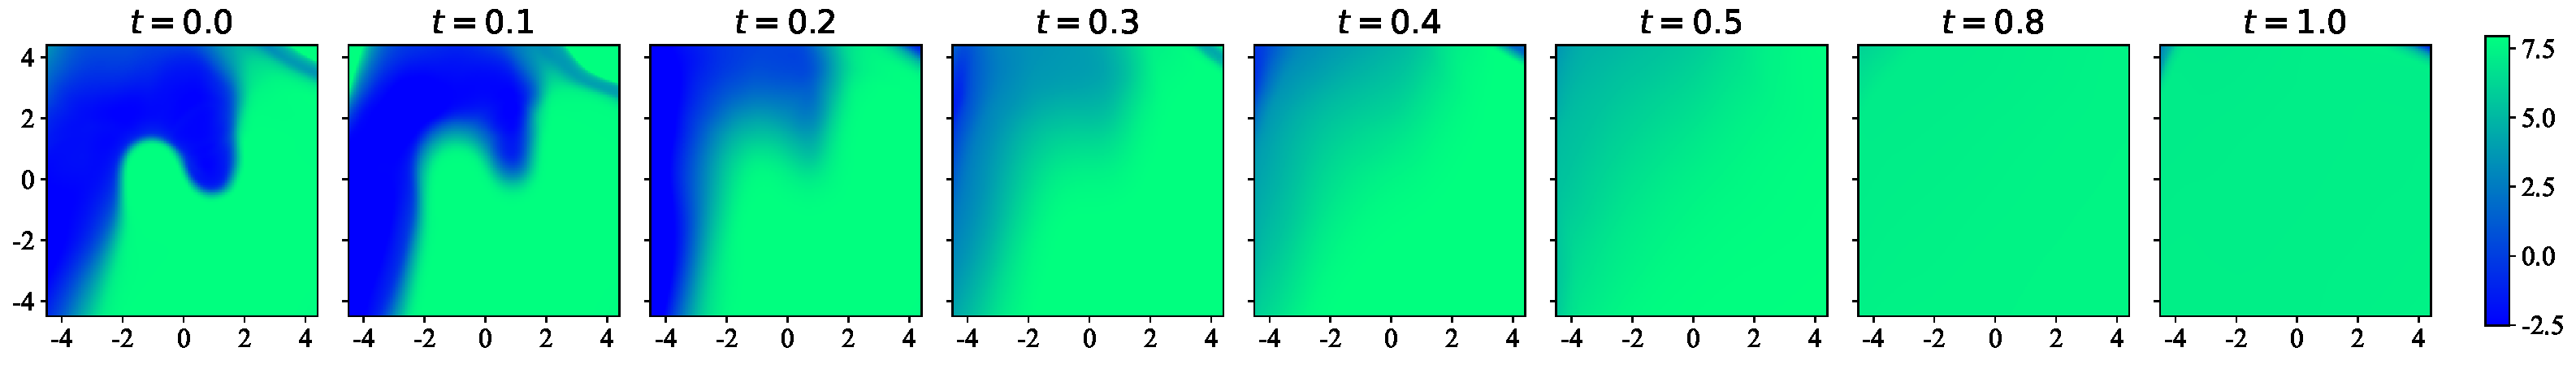
\includegraphics[width=\columnwidth]{pics/toy_scatter/moons_qt.pdf}
\end{minipage}\\
\begin{minipage}{0.02\linewidth}
\rotatebox{90}{\scriptsize{rings}}
\end{minipage}
\begin{minipage}{0.97\linewidth}
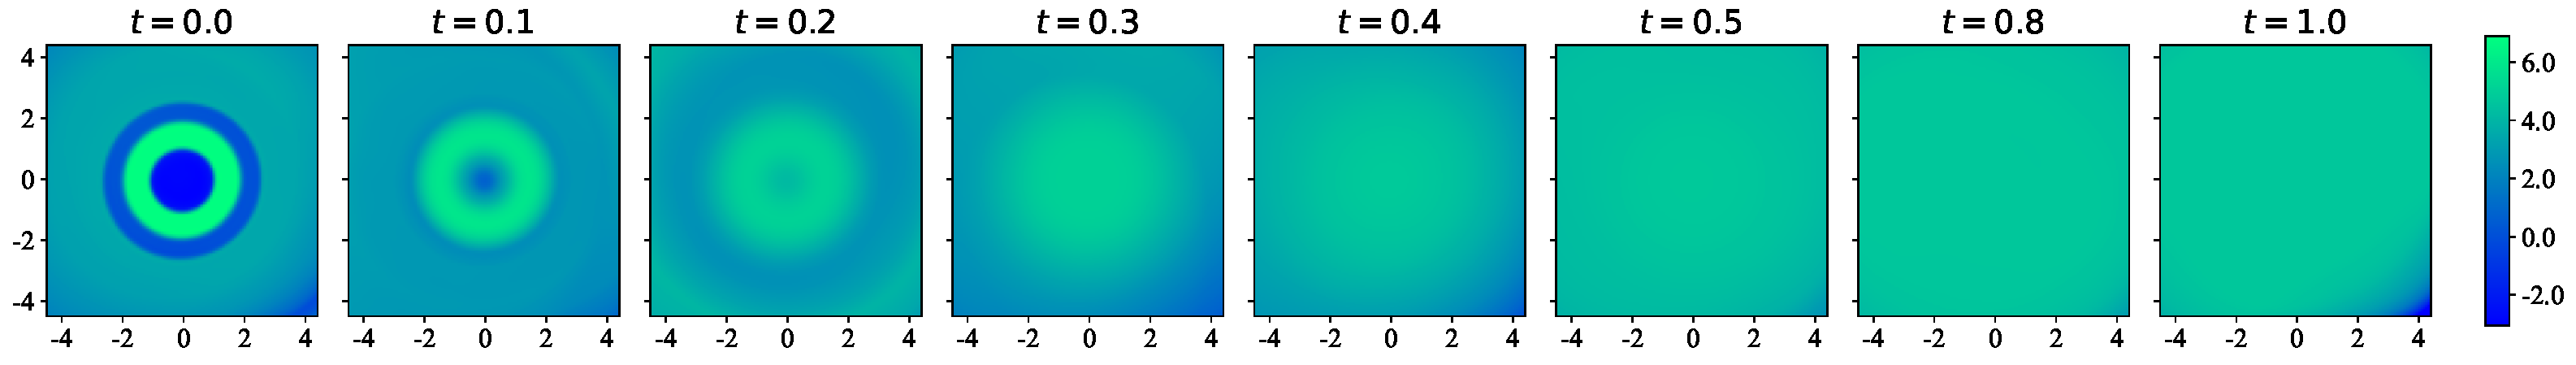
\includegraphics[width=\columnwidth]{pics/toy_scatter/rings_qt.pdf}
\end{minipage}\\
\caption{Visualization of the contrastively learned intermediate energy model when $\beta=10$.}
\vspace{-8mm}
\label{fig:toy_appendix_qt}
\end{figure}


\newpage


\newpage
\section{Training Curves for Offline Reinforcement Learning}
\label{sec:training_curves}
\begin{figure}[!h]
\vspace{-2mm}
\centering
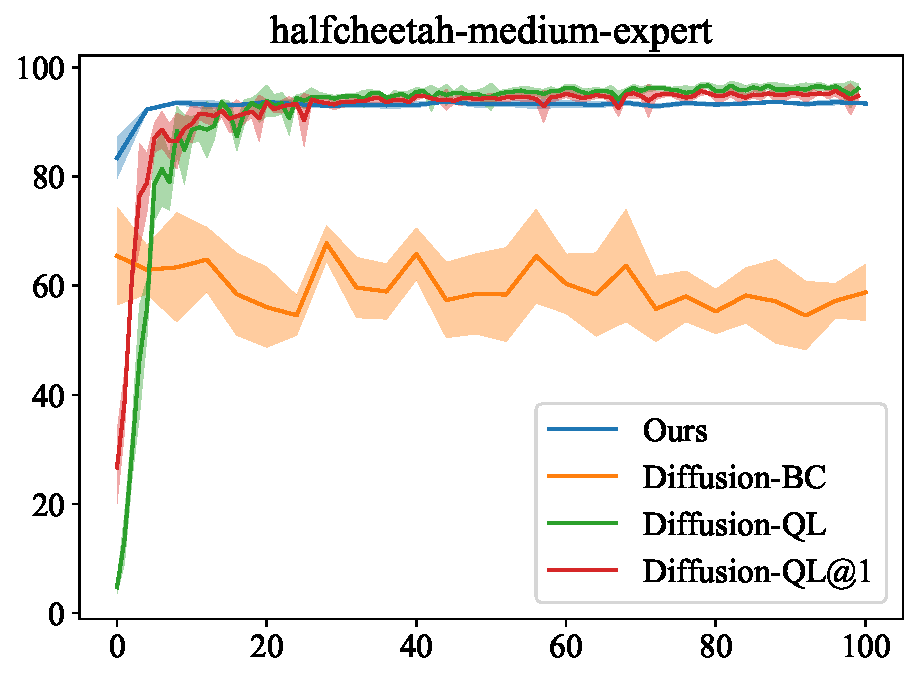
\includegraphics[width = .33\linewidth]{pics/plots/halfcheetah-medium-expert-v2_plot.pdf}
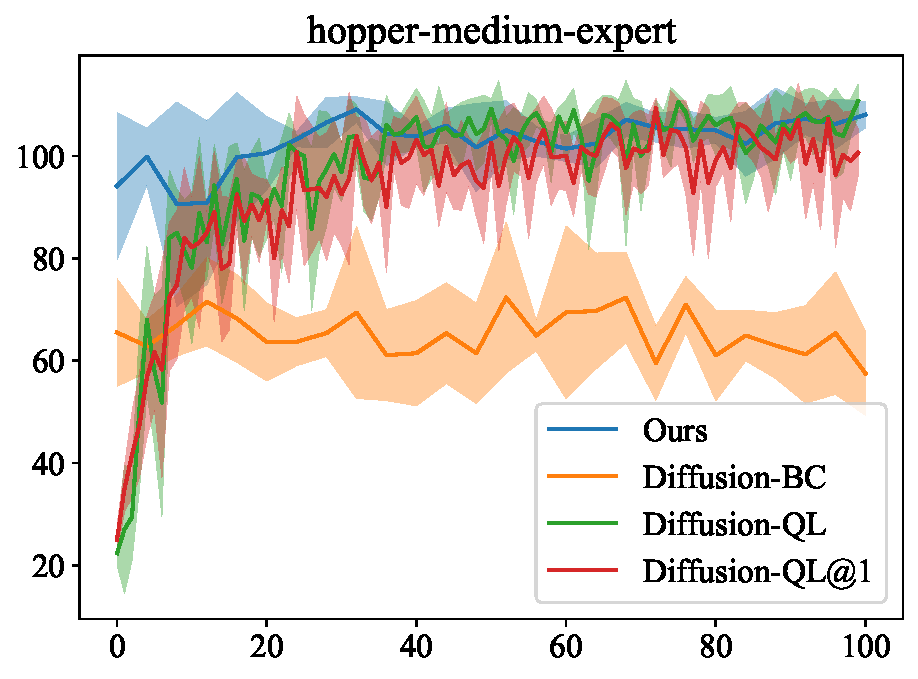
\includegraphics[width = .33\linewidth]{pics/plots/hopper-medium-expert-v2_plot.pdf}
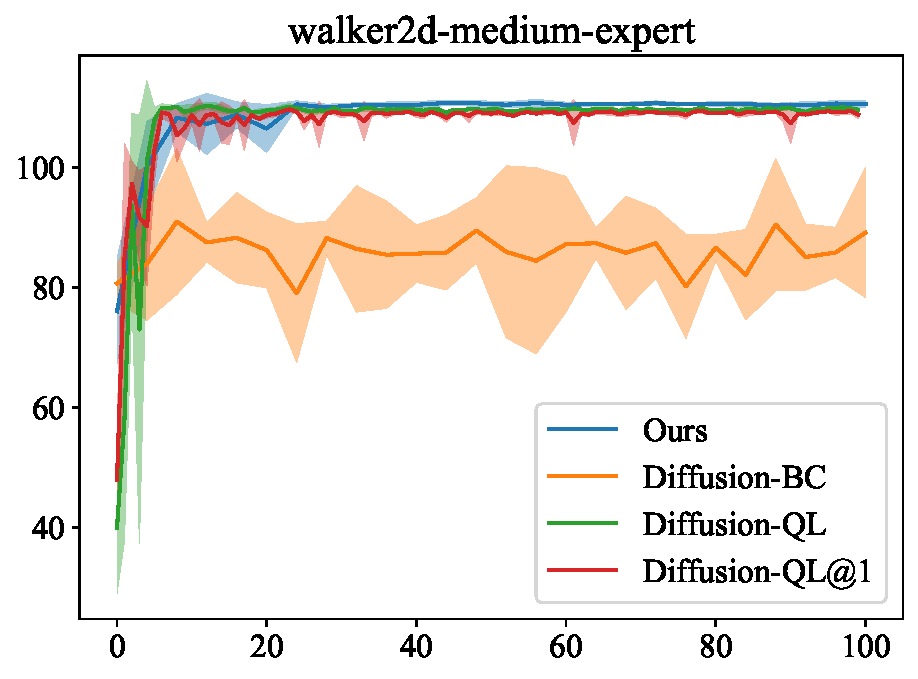
\includegraphics[width = .33\linewidth]{pics/plots/walker2d-medium-expert-v2_plot.pdf}\\
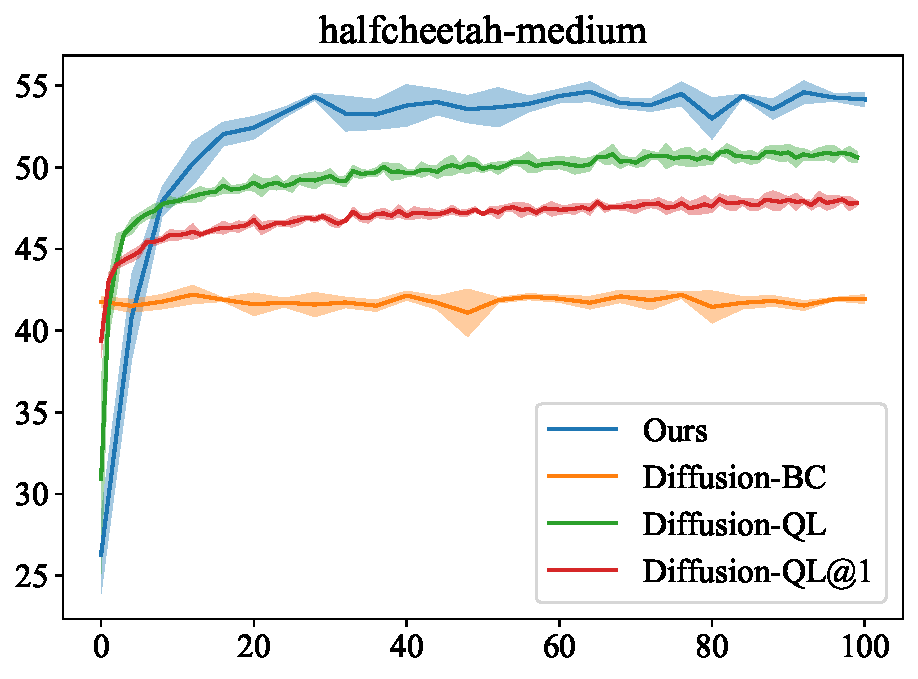
\includegraphics[width = .33\linewidth]{pics/plots/halfcheetah-medium-v2_plot.pdf}
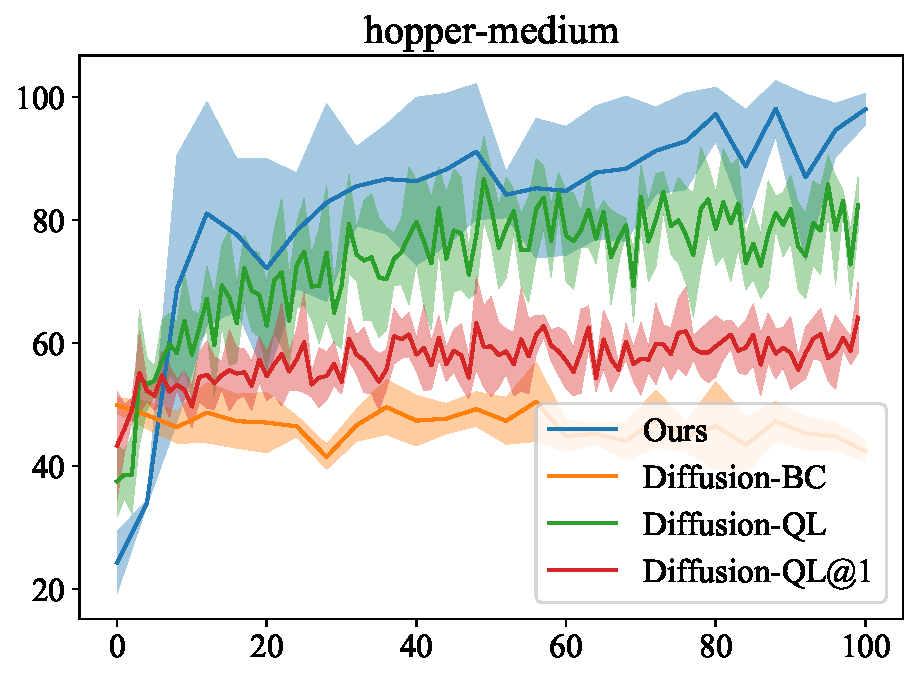
\includegraphics[width = .33\linewidth]{pics/plots/hopper-medium-v2_plot.pdf}
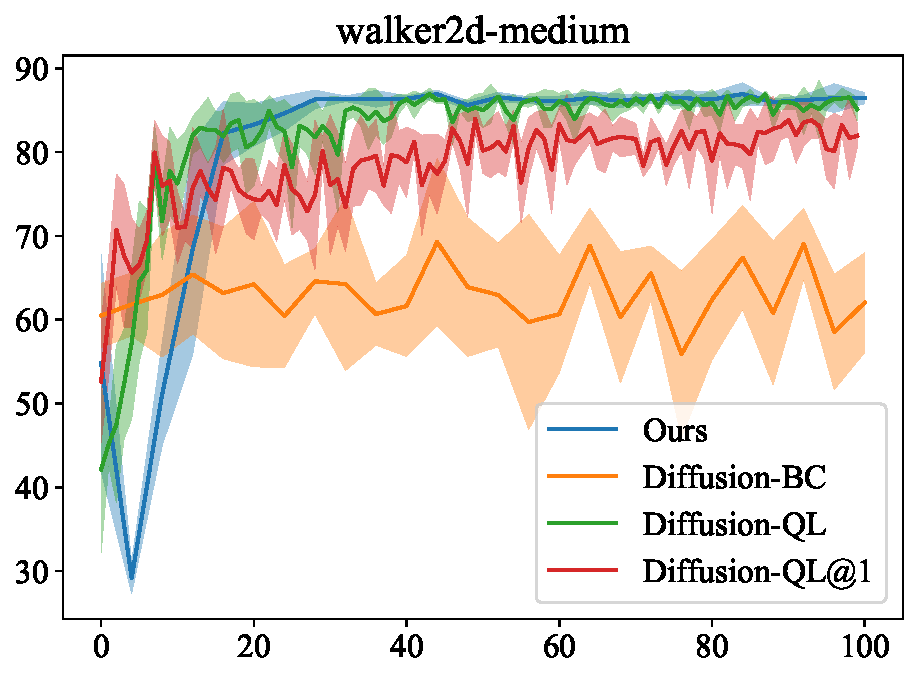
\includegraphics[width = .33\linewidth]{pics/plots/walker2d-medium-v2_plot.pdf}\\
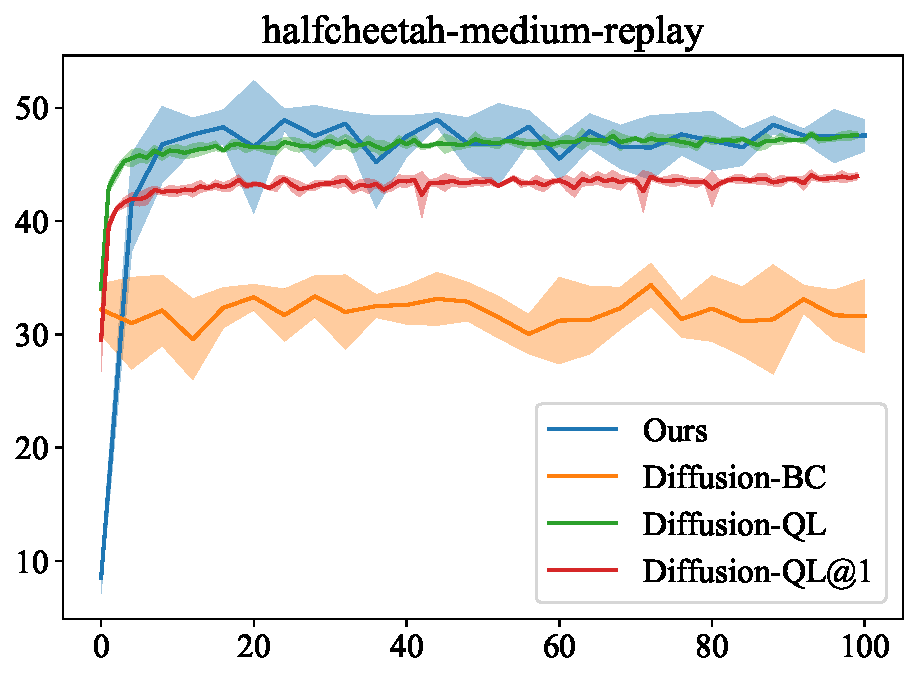
\includegraphics[width = .33\linewidth]{pics/plots/halfcheetah-medium-replay-v2_plot.pdf}
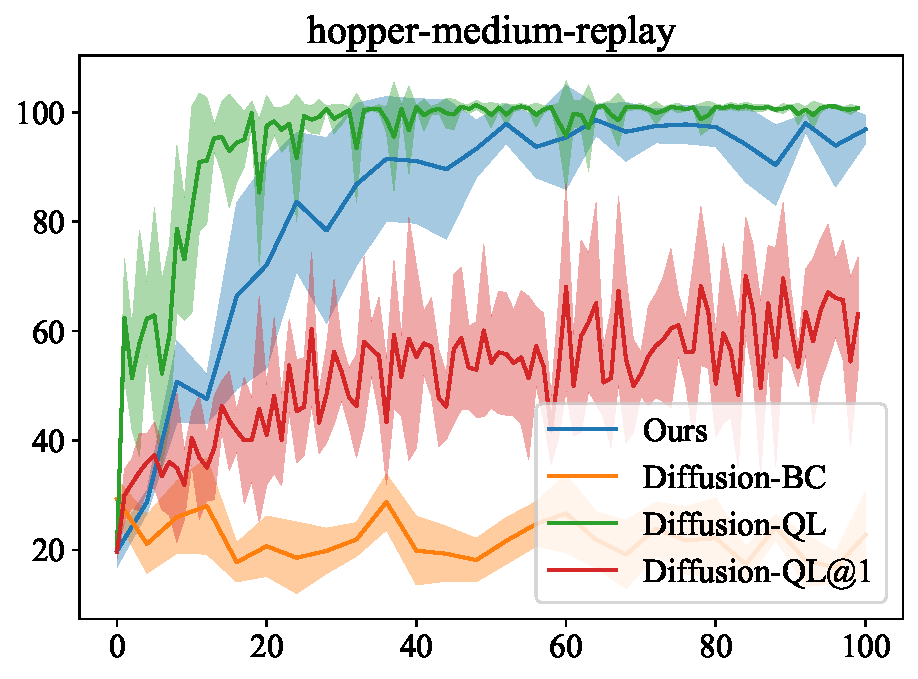
\includegraphics[width = .33\linewidth]{pics/plots/hopper-medium-replay-v2_plot.pdf}
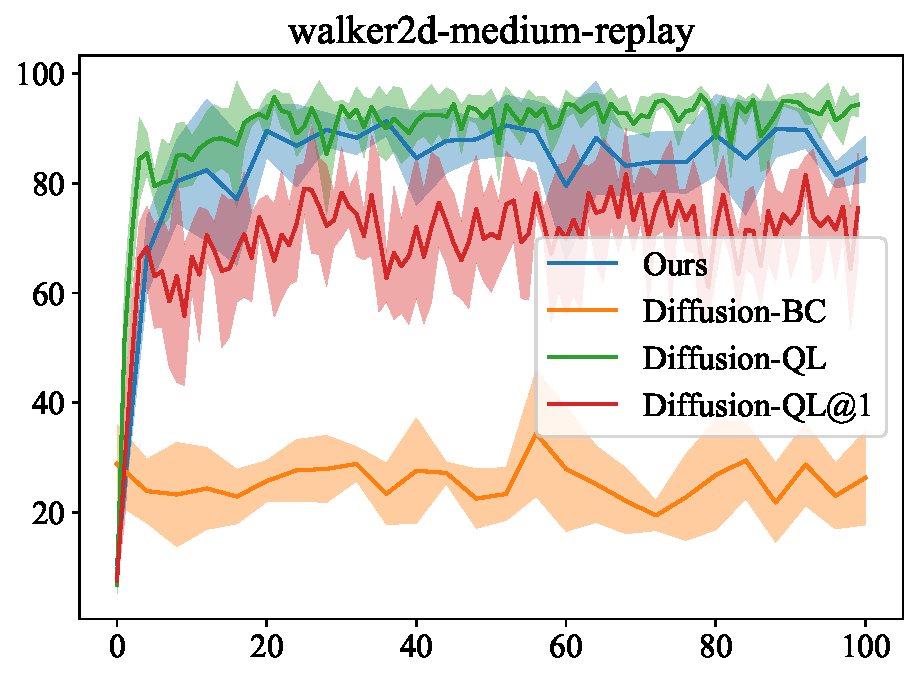
\includegraphics[width = .33\linewidth]{pics/plots/walker2d-medium-replay-v2_plot.pdf}\\
\includegraphics[width = .33\linewidth]{pics/plots/AntMaze-umaze-v0_plot.pdf}
\includegraphics[width = .33\linewidth]{pics/plots/AntMaze-umaze-diverse-v0_plot.pdf}
\includegraphics[width = .33\linewidth]{pics/plots/AntMaze-medium-diverse-v0_plot.pdf}\\
\includegraphics[width = .33\linewidth]{pics/plots/AntMaze-medium-play-v0_plot.pdf}
\includegraphics[width = .33\linewidth]{pics/plots/AntMaze-large-diverse-v0_plot.pdf}
\includegraphics[width = .33\linewidth]{pics/plots/AntMaze-large-play-v0_plot.pdf}\\
\vspace{-2mm}
\caption{Training curves of QGPO (ours) and several baselines. We plot mean and standard deviation of results across five random seeds. Scores are normalized according to \cite{d4rl}. Diffusion BC indicates evaluation scores of the learned behavior policy without any guidance ($s=0$).}
\vspace{-4mm}
\label{fig:plots}
\end{figure}

\newpage
\section{More Results for Energy-Guided Image Synthesis}
\label{Sec:Scale_samples}
\begin{figure}[hbt!]
\centering
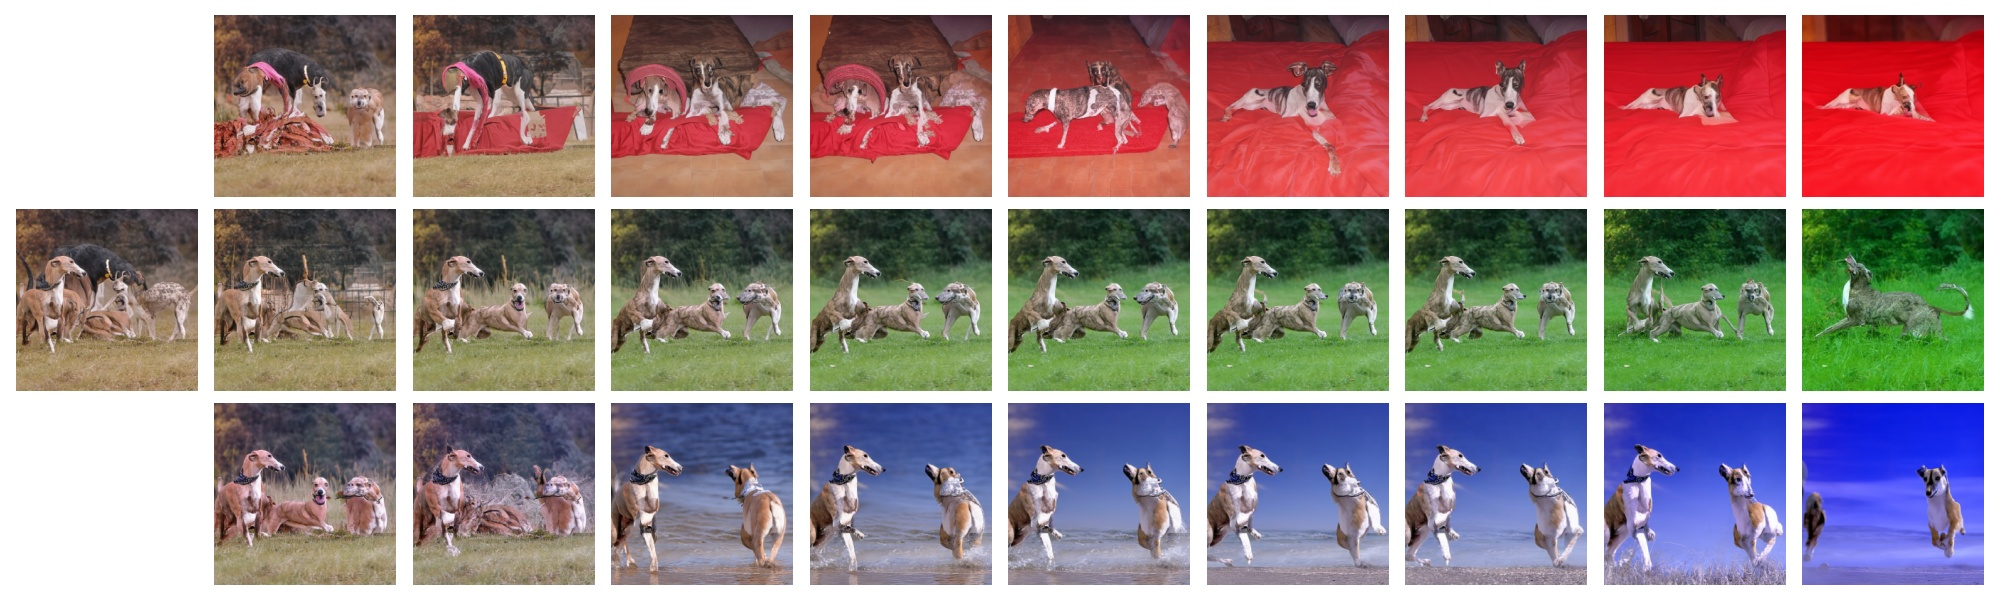
\includegraphics[width = 0.94\linewidth]{pics/color_imgs/cond_3.jpg}
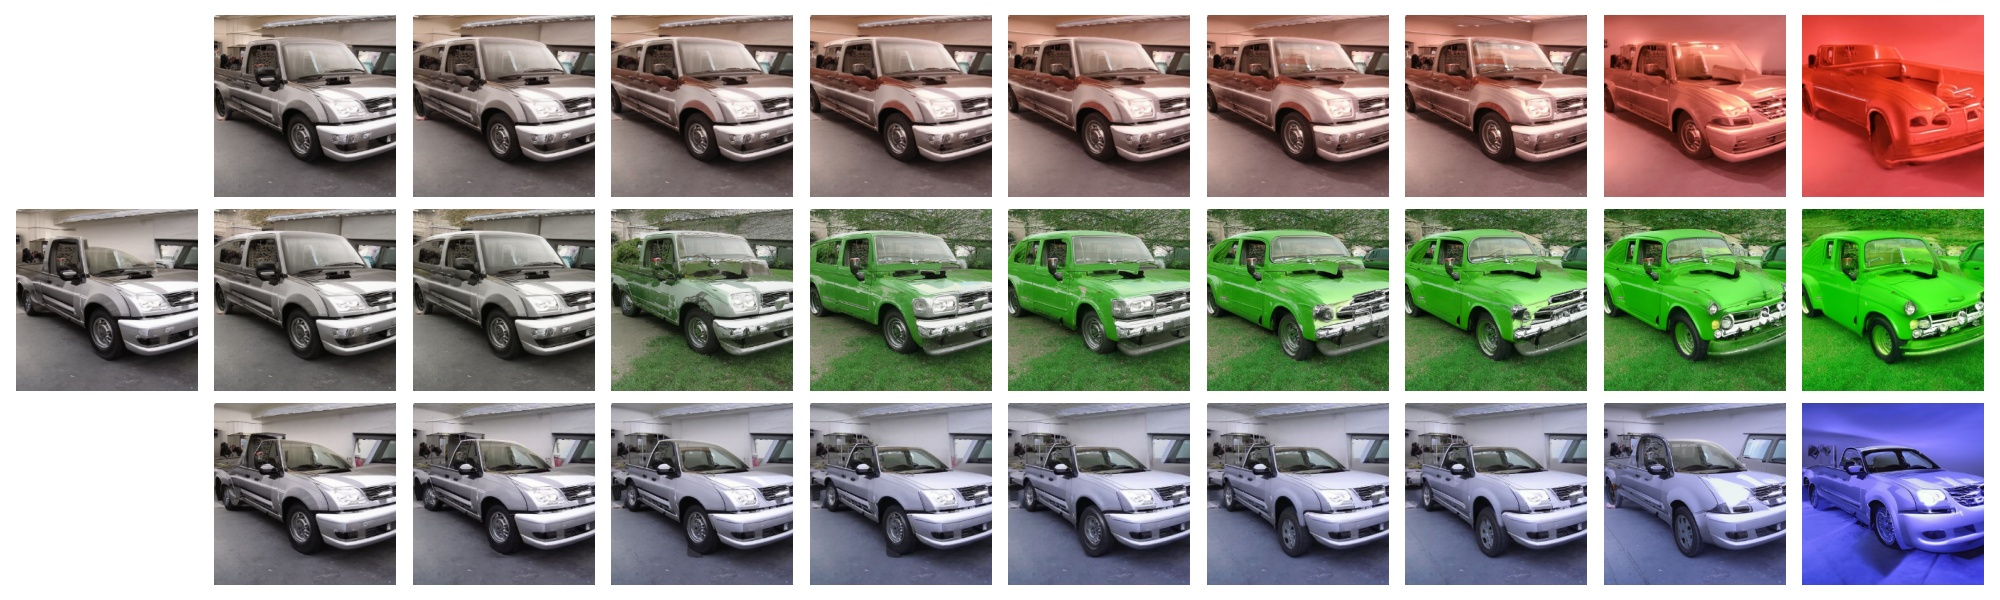
\includegraphics[width = 0.94\linewidth]{pics/color_imgs/cond_11.jpg}
\vspace{-3mm}
\caption{Ablation of color guidance with a conditional diffusion prior. From left to right are samples under an increasing guidance scale in [0.0, 0.25, 0.5, 1.0, 1.5, 2.0, 2.5, 3.0, 5.0, 10.0].}
\label{fig:colors_conditional}
\end{figure}
\begin{figure}[hbt!]
\centering
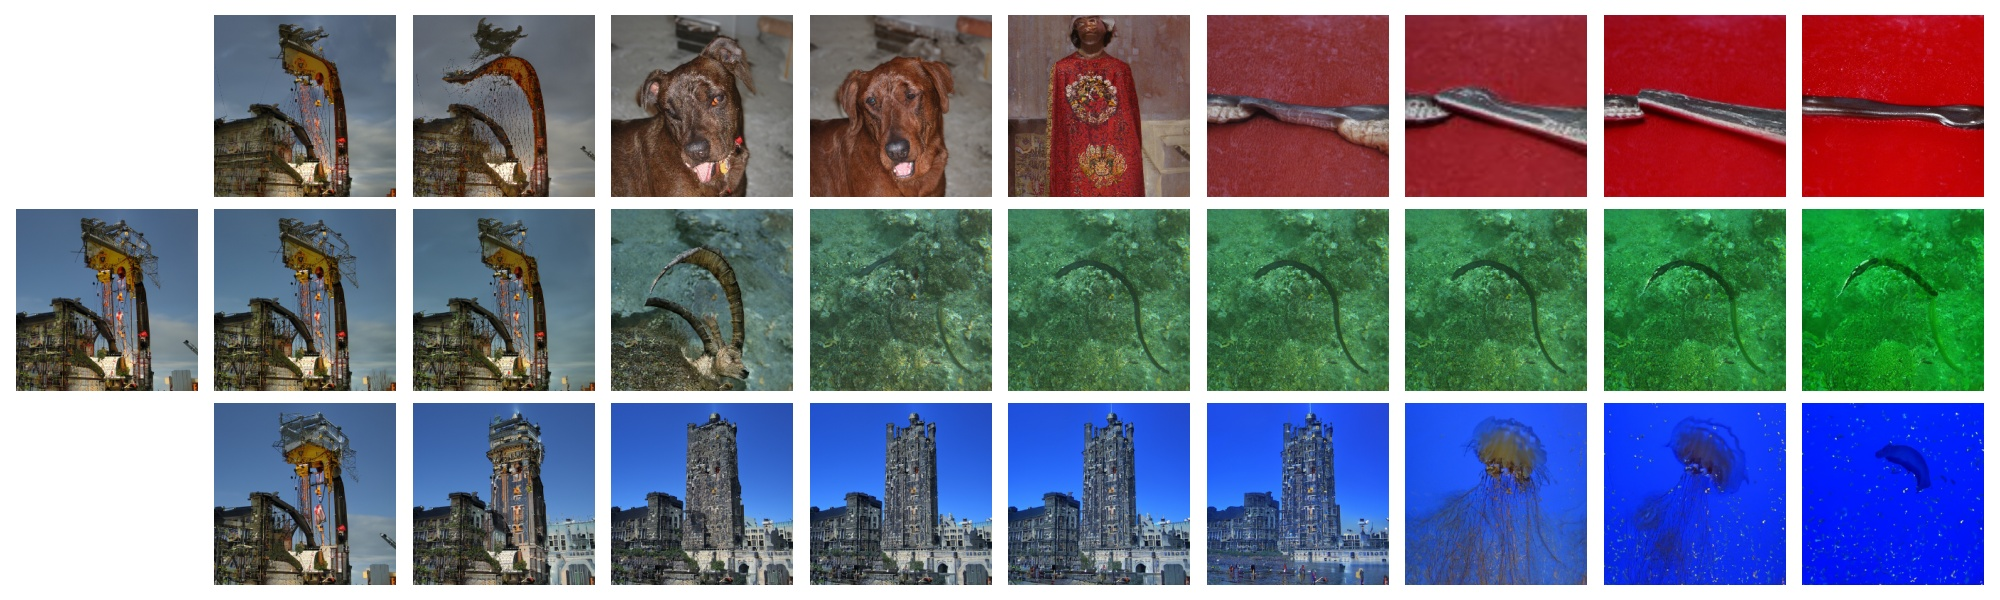
\includegraphics[width = 0.94\linewidth]{pics/color_imgs/uncond_50.jpg}
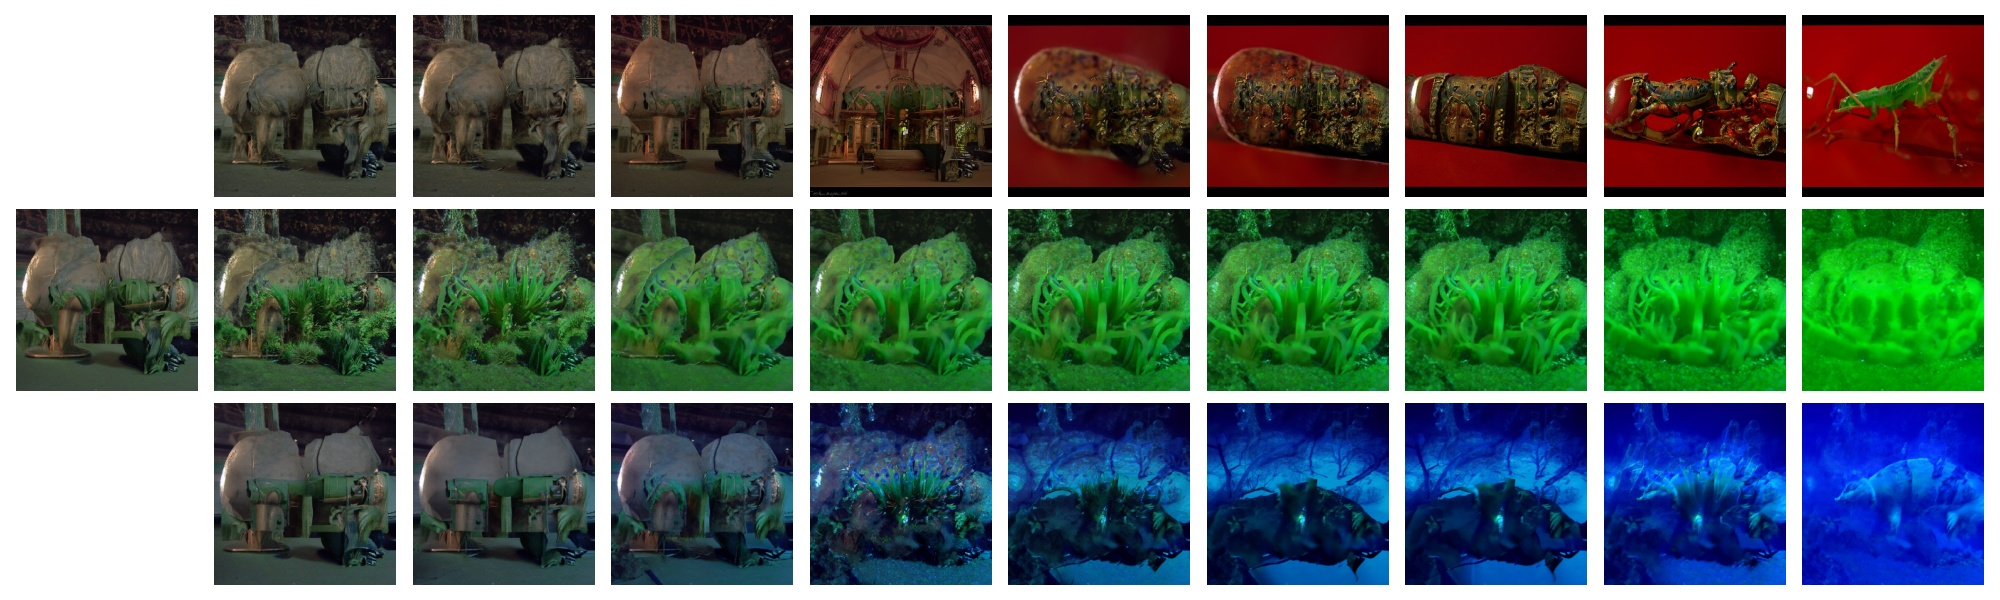
\includegraphics[width = 0.94\linewidth]{pics/color_imgs/uncond_1.jpg}
\vspace{-3mm}
\caption{Ablation of color guidance with an unconditional diffusion prior. From left to right are samples under an increasing guidance scale in [0.0, 0.25, 0.5, 1.0, 1.5, 2.0, 2.5, 3.0, 5.0, 10.0].}
\label{fig:colors}
\end{figure}

\newpage
\section{CEP Guidance vs. Classifier Guidance}
\label{fig:image_guidance_qualitative}
\begin{figure}[!hbt]
\centering
\vspace{-2mm}
\begin{minipage}{0.48\linewidth}
\centering
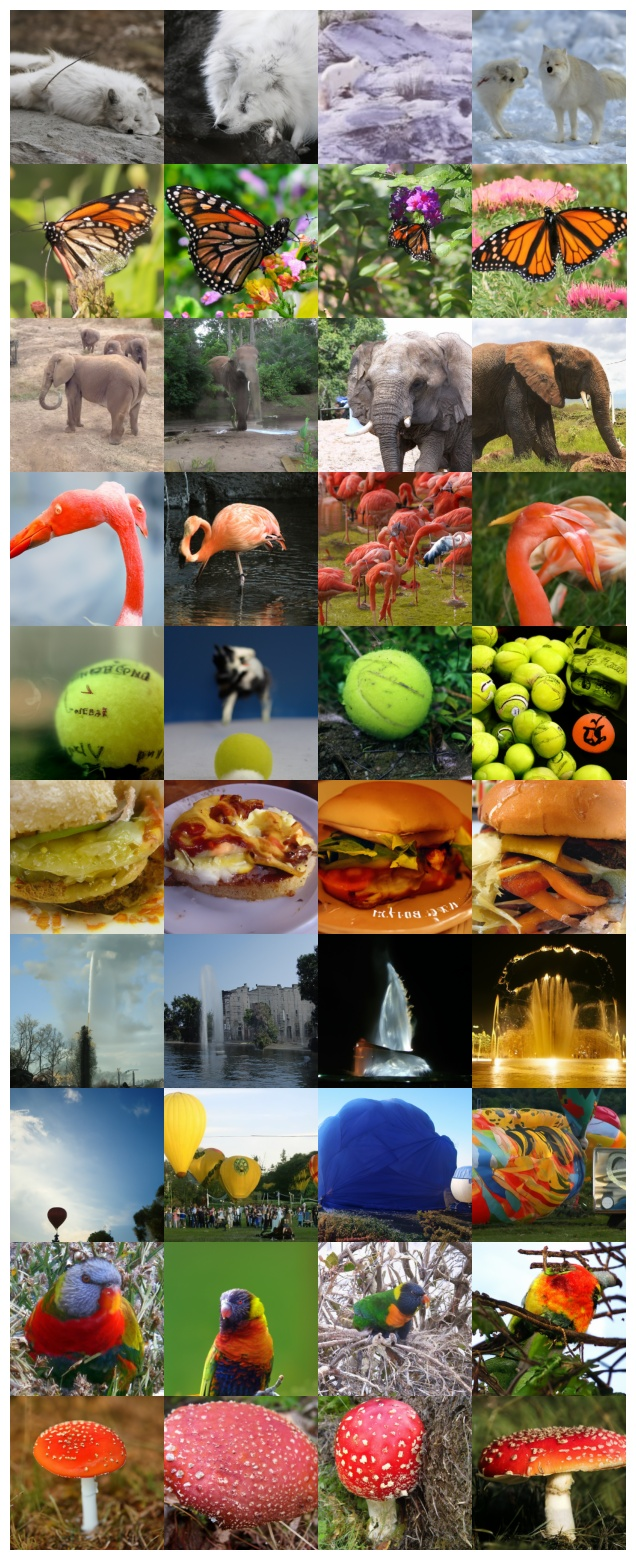
\includegraphics[width =\linewidth]{pics/guided_diffusion_imagenet256_sample.jpg}
Classifier guidance \citep{diffusion_beat_gan} \\
\end{minipage}
\begin{minipage}{0.48\linewidth}
\centering
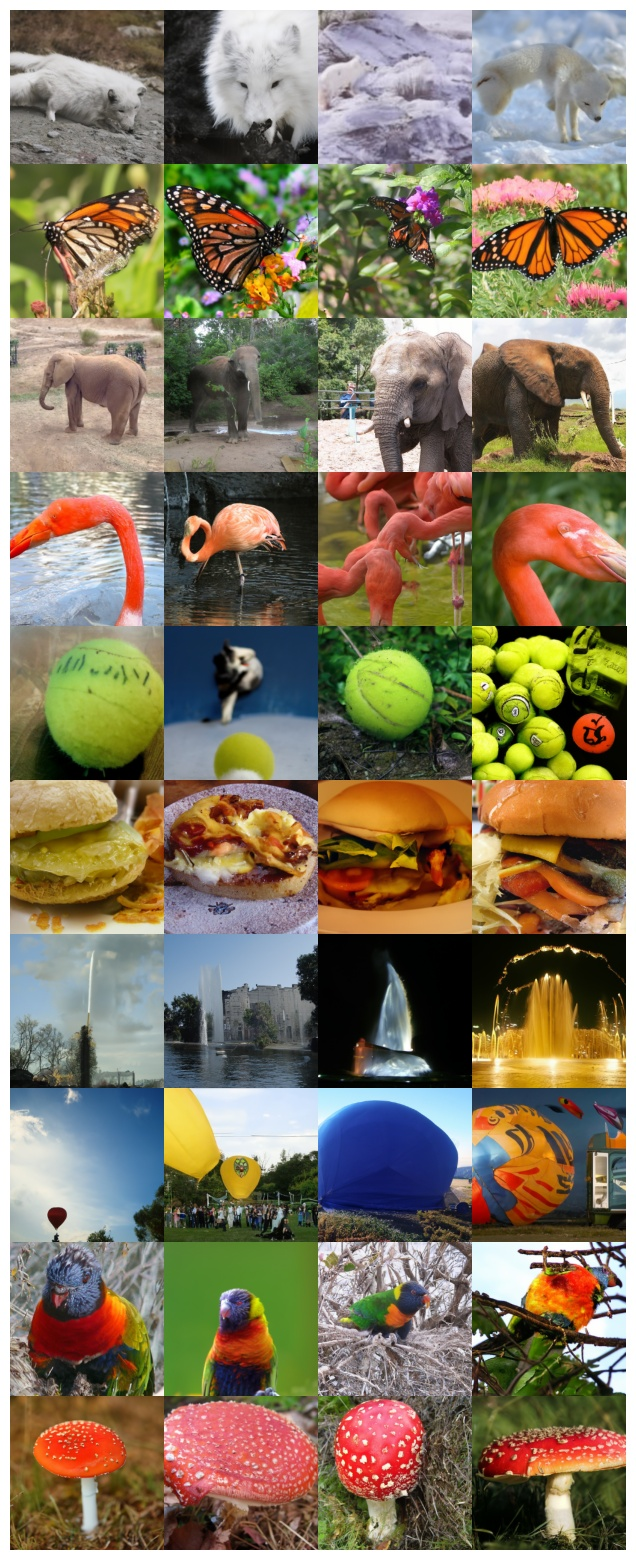
\includegraphics[width =\linewidth]{pics/contrastive_imagenet256_sample.jpg}
Energy guidance (\textbf{ours}) \\
\end{minipage}
\caption{Samples from the conditional 256×256 ImageNet model with different guidance methods. Random seeds are fixed across experiments. Classes are 279: arctic fox, 323: monarch butterfly, 386: african elephant, 130: flamingo, 852: tennis ball, 933: cheeseburger, 562: fountain, 417: balloon, 90: lorikeet, 992: agaric.}
\vspace{-8mm}
\end{figure}